\documentclass[11pt,letterpaper]{article}
\usepackage{fontspec}
\setmainfont{texgyrepagella}[Extension=.otf,UprightFont=*-regular,BoldFont=*-bold,ItalicFont=*-italic,BoldItalicFont=*-bolditalic]
\usepackage[bidi=default]{babel}
\babelprovide[import,main]{spanish}
\babelprovide[import]{hebrew}
\babelprovide[import]{ancientgreek}
\babelfont[hebrew]{rm}[Path=fonts/,BoldFont=NotoHebrewSerif-700.ttf,Scale=0.95]{NotoHebrewSerif-400.ttf}
\babelfont[ancientgreek]{rm}[Path=fonts/]{GFSPorson.otf}
\newcommand{\heb}[1]{\mbox{\foreignlanguage{hebrew}{#1}}}
\newcommand{\grc}[1]{\foreignlanguage{ancientgreek}{#1}}
\newcommand{\hebverso}[1]{\par\smallskip{\centering\begin{otherlanguage}{hebrew}\large #1\end{otherlanguage}\par}\smallskip}
\newcommand{\SENOR}{\textsc{Señor}}
\usepackage[margin=2.5cm,headheight=14pt]{geometry}
\usepackage{microtype,ragged2e,booktabs,graphicx,xcolor,csquotes,array}
\usepackage[hidelinks]{hyperref}\usepackage{xurl}\urlstyle{same}
\usepackage[most]{tcolorbox}
\usepackage{tikz}\usetikzlibrary{arrows.meta,positioning,calc,decorations.pathreplacing,shapes.geometric}
\usepackage{titlesec,fancyhdr}
\definecolor{tierraroja}{RGB}{122,40,18}\definecolor{caferojizo}{RGB}{58,18,8}
\definecolor{mostaza}{RGB}{214,160,58}\definecolor{papiro}{RGB}{243,228,192}\definecolor{sepia}{RGB}{98,66,44}
\definecolor{oliva}{RGB}{92,98,48}
\titleformat{\section}{\Large\bfseries\color{tierraroja}}{\thesection.}{0.6em}{}
\titleformat{\subsection}{\large\bfseries\color{caferojizo}}{\thesubsection}{0.6em}{}
\pagestyle{fancy}\fancyhf{}
\fancyhead[L]{\foreignlanguage{spanish}{\small\itshape\color{sepia}Yom Teruá}}\fancyhead[R]{\foreignlanguage{spanish}{\small\color{sepia}\thepage}}
\renewcommand{\headrulewidth}{0.4pt}
\setlength{\parindent}{1.27cm}\linespread{1.15}\setlength{\emergencystretch}{3em}
\newtcolorbox{cita}[1][]{enhanced,unbreakable,colback=tierraroja!5!white,colframe=tierraroja,boxrule=0pt,leftrule=2.5pt,arc=0pt,
  left=8pt,right=8pt,top=5pt,bottom=5pt,before skip=8pt,after skip=8pt,fontupper=\itshape,#1}
\newcommand{\fuente}[1]{\par\hfill{\upshape\bfseries\small\textcolor{tierraroja}{#1}}}
\newtcolorbox{nota}[1][]{enhanced,unbreakable,colback=mostaza!10,colframe=mostaza!85!tierraroja,boxrule=0.6pt,arc=2pt,
  fonttitle=\bfseries\small,coltitle=caferojizo,colbacktitle=mostaza!30,fontupper=\small,title={#1}}
\newtcolorbox{filologia}[1][]{enhanced,unbreakable,colback=white,colframe=tierraroja!45,boxrule=0.5pt,arc=2pt,
  fonttitle=\bfseries\small,coltitle=white,colbacktitle=tierraroja!80,fontupper=\small,title={Filología: #1}}
\newcommand{\refapa}[1]{\par{\RaggedRight\hangindent=1.27cm\hangafter=1\noindent #1\par}\vspace{4pt}}
\newcommand{\destacar}[1]{\textbf{\textcolor{tierraroja}{#1}}}
\newcolumntype{L}[1]{>{\RaggedRight\arraybackslash}p{#1}}

\title{\color{tierraroja}\bfseries Yom Teruá: el día del sonido de trompeta\\[4pt]\large\color{sepia}\mdseries ``Una conmemoración al son de trompetas, y una santa convocación'' (Lv 23:24)}
\author{}\date{}
\begin{document}
\maketitle\thispagestyle{empty}

\begin{abstract}\noindent
Levítico 23 dedica a la quinta convocación solo tres versículos: el primer día del mes séptimo será \emph{shabatón}, \emph{zijrón teruá} y \emph{mikrá kódesh}, con ofrenda encendida (Lv 23:23--25). Números la llama \emph{yom teruá}, ``día de sonar las trompetas'' (Nm 29:1), y tampoco dice qué acontecimiento recuerda. Este capítulo estudia la fiesta con el método de la serie. En lo histórico, el mes séptimo (Etanim o Tishri) al final del ciclo agrícola, las dos trompetas de plata y el cuerno de carnero, el Sinaí, Jericó, el altar de Esdras y la lectura de la Torá en Nehemías 8. En lo filológico, \emph{teruá}, \emph{shofar}, \emph{jatsotsrá}, \emph{yovel}, \emph{taqa'}, \emph{zikarón}, \emph{shabatón} y \emph{kese}, junto con la Septuaginta y el griego del Nuevo Testamento. En lo textual, qué instrumento supone Lv 23, el debate de Sal 81:3 [81:4] y el ``año nuevo'' que la Biblia no nombra así. En lo literario, la trompeta en el canon, desde el Sinaí hasta las siete trompetas del Apocalipsis. La lectura de la serie ocupa una sección propia: la ``conmemoración'' remite a la caída de Jericó, y para la Iglesia la fiesta anuncia el regreso de Cristo a la final trompeta para establecer su Reino y congregar a su pueblo (1~Co 15:51--53; 1~Ts 4:15--17; Ap 10:7; 11:15). Donde el texto lo exige se agregan precisiones, en particular que Lv 23 no menciona Jericó y que Josué fecha la caída de la ciudad en el mes primero. El capítulo cierra con la tradición judía, las posturas de interpretación y una síntesis.
\par\smallskip\noindent\textbf{Palabras clave:} Yom Teruá, Fiesta de las Trompetas, \emph{teruá}, \emph{shofar}, \emph{zijrón}, Jericó, Rosh haShaná, final trompeta, Apocalipsis 8--11.\end{abstract}

\begin{nota}[Nota sobre el texto]
Las citas bíblicas en español son de la Reina-Valera 1960, convención vigente de la serie; donde esta escribe ``Jehová'', aquí se escribe \SENOR, que traduce el tetragrama \heb{יהוה}. Cuando no hay certeza de la redacción exacta, el texto se parafrasea sin comillas o se marca como traducción propia. El hebreo sigue la BHS; el griego, NA28 y la Septuaginta de Rahlfs-Hanhart. La numeración hebrea, cuando difiere, va entre corchetes: Sal 81:3 [81:4]. Las fuentes judías (Misná, Talmud, Rashi, Maimónides) se citan desde Sefaria y la traducción de Danby (1933); lo que es tradición, tipología, cálculo o hipótesis se marca como \emph{precisión}. Los conteos de palabras son propios y deben verificarse en la BHS o e-Sword. Integro aquí mis dos presentaciones anteriores sobre la fiesta (``Yom Teruá'' y ``La fiesta del séptimo mes''); la referencia ``Éxodo 23:23--25'' de una de esas láminas corresponde a Lv 23:23--25.
\end{nota}

%===================================================================
\section{Introducción: una fiesta que solo se oye}

De las siete convocaciones de Levítico 23, la quinta es la más breve y la que menos explica de sí misma. Pésaj recuerda la noche de Egipto; Sukkot, las cabañas del desierto (Lv 23:43); Yom Kipur tiene un capítulo entero de ritual (Lv 16). Al primer día del mes séptimo la ley le da nombre, fecha, reposo y ofrenda, pero no dice qué hecho conmemora ni qué debe sentir el pueblo. Dice que será \destacar{zijrón teruá}, ``una conmemoración al son de trompetas'' (Lv 23:24), y Números lo resume todavía más: \emph{yom teruá yihyé lajem}, ``os será día de sonar las trompetas'' (Nm 29:1). Lo único que la Torá fija de este día es un sonido.

Esa reticencia del texto explica por qué la fiesta ha recibido tantas lecturas. El judaísmo rabínico la convirtió en \emph{Rosh haShaná}, el año nuevo y el día del juicio, que abre diez días de arrepentimiento hasta Yom Kipur. Filón de Alejandría la vio como memoria del Sinaí. El documento de referencia de esta serie pregunta por qué el texto dice ``conmemoración'' y responde con un hito de la historia de Israel, la caída de Jericó al son de las trompetas; para la Iglesia, la fiesta señala el regreso de Cristo ``a la final trompeta'' (1~Co 15:52). Otras lecturas cristianas ven en ella el arrebatamiento de la Iglesia o el día del \SENOR{} anunciado por los profetas.

Sostengo en este estudio que la Escritura misma explica el sentido de la \emph{teruá}, y que lo hace en dos direcciones. Hacia atrás, Números 10 enseña que el sonido de las trompetas hace que Israel ``sea recordado'' delante de Dios en la guerra y en las fiestas (Nm 10:9--10); la memoria, antes que del pueblo, es de Dios. Hacia adelante, los profetas convierten el \emph{shofar} en la señal del día del \SENOR{} y de la reunión de los dispersos (Jl 2:1; Sof 1:16; Is 27:13), y los apóstoles oyen en esa misma trompeta el anuncio de la venida de Cristo y de la resurrección (Mt 24:31; 1~Co 15:52; 1~Ts 4:16; Ap 11:15). La lectura de la serie, que vincula la fiesta con Jericó y con el regreso de Cristo, se inscribe en esa trayectoria; la expongo con fidelidad y marco dónde es tipología y dónde es texto.

El recorrido sigue el orden habitual de la serie: el texto (§2), la historia (§3), la filología (§4), las cuestiones textuales y de calendario (§5), la forma literaria (§6), la lectura de la serie (§7), la fiesta en Jesús y los apóstoles (§8), la tradición judía (§9), la discusión de interpretaciones (§10) y la síntesis (§11--12). La Figura~1 sitúa la fiesta en el ciclo de Lv 23.

\begin{center}\begin{minipage}{\linewidth}\centering
% === Esquema estándar de la serie: el ciclo de Levítico 23 ===
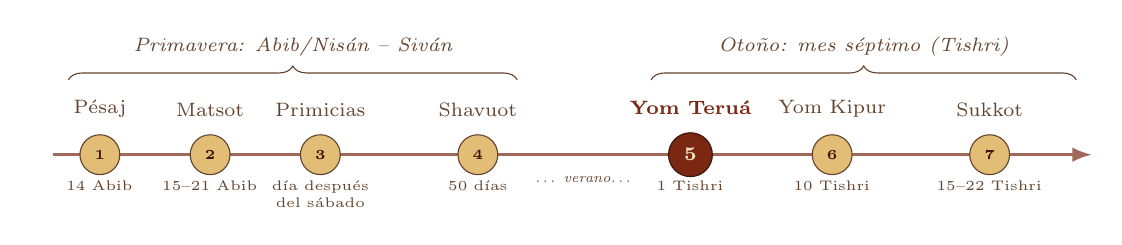
\begin{tikzpicture}[x=1cm,y=1cm,font=\scriptsize]
 \def\fiestaactual{5}
 \draw[line width=1.2pt,tierraroja!70,-{Latex[length=2.5mm]}] (0,0) -- (13.2,0);
 \draw[decorate,decoration={brace,amplitude=5pt},sepia] (0.2,0.95) -- (5.9,0.95) node[midway,above=5pt,font=\scriptsize\itshape]{Primavera: Abib/Nisán -- Siván};
 \draw[decorate,decoration={brace,amplitude=5pt},sepia] (7.6,0.95) -- (13.0,0.95) node[midway,above=5pt,font=\scriptsize\itshape]{Otoño: mes séptimo (Tishri)};
 \foreach \n/\x/\t/\d in {1/0.6/Pésaj/{14 Abib},2/2.0/Matsot/{15--21 Abib},3/3.4/Primicias/{día después del sábado},4/5.4/Shavuot/{50 días},5/8.1/Yom Teruá/{1 Tishri},6/9.9/Yom Kipur/{10 Tishri},7/11.9/Sukkot/{15--22 Tishri}}{
   \ifnum\n=\fiestaactual
     \node[circle,fill=tierraroja,draw=caferojizo,minimum size=5.5mm,text=papiro,font=\scriptsize\bfseries] at (\x,0) {\n};
     \node[above=3pt,font=\scriptsize\bfseries,text=tierraroja] at (\x,0.28) {\t};
   \else
     \node[circle,fill=mostaza!70,draw=sepia,minimum size=4.5mm,text=caferojizo,font=\tiny\bfseries] at (\x,0) {\n};
     \node[above=3pt,text=sepia] at (\x,0.25) {\t};
   \fi
   \node[below=6pt,text width=1.6cm,align=center,font=\tiny,text=sepia] at (\x,0) {\d};}
 \node[font=\tiny\itshape,text=sepia] at (6.75,-0.32) {\ldots\ verano\ldots};
\end{tikzpicture}\par
{\footnotesize\color{sepia}\textit{Figura 1.} El ciclo de las convocaciones de Levítico 23; resaltada, Yom Teruá. \textit{Nota.} Elaboración propia, esquema estándar de la serie.}
\end{minipage}\end{center}

%===================================================================
\section{El texto: tres versículos y un nombre}

\subsection{Levítico 23:23--25}
La unidad abre con la fórmula que separa cada bloque de Lv 23 (``Y habló \SENOR{} a Moisés''), y contiene en un solo versículo los cuatro rasgos de la fiesta:

\hebverso{דַּבֵּר אֶל־בְּנֵי יִשְׂרָאֵל לֵאמֹר בַּחֹדֶשׁ הַשְּׁבִיעִי בְּאֶחָד לַחֹדֶשׁ \\ יִהְיֶה לָכֶם שַׁבָּתוֹן זִכְרוֹן תְּרוּעָה מִקְרָא־קֹדֶשׁ}
\begin{cita}Y habló \SENOR{} a Moisés, diciendo: Habla a los hijos de Israel y diles: En el mes séptimo, al primero del mes tendréis día de reposo, una conmemoración al son de trompetas, y una santa convocación. Ningún trabajo de siervos haréis; y ofreceréis ofrenda encendida a \SENOR.\fuente{(Lv 23:23--25)}\end{cita}

La sintaxis hebrea es nominal y escueta. Después de la fecha (``en el mes séptimo, en el uno del mes'') vienen tres sustantivos en aposición: \heb{שַׁבָּתוֹן} (\emph{shabatón}, ``reposo solemne''), \heb{זִכְרוֹן תְּרוּעָה} (\emph{zijrón teruá}, literalmente ``memoria de clamor'' o ``recordación de toque'') y \heb{מִקְרָא־קֹדֶשׁ} (\emph{mikrá kódesh}, ``convocación santa''). El versículo 25 agrega dos órdenes que comparten varias fiestas: no hacer \emph{mlejet avodá} (``trabajo de servicio'', el trabajo ordinario) y presentar \heb{אִשֶּׁה} (\emph{ishé}, ``ofrenda encendida''). Lv 23 no detalla la ofrenda ni nombra el instrumento; donde la RVR1960 lee ``al son de trompetas'' el hebreo dice \emph{teruá}, un sonido o un grito. La versión interpreta a partir de Nm 10:10 y de la tradición, y con buena razón, como veremos en §5.1.

\subsection{Números 29:1--6}
Números 28--29 es el calendario de ofrendas públicas, lo que el documento de referencia llama, con Pablo, la ley de los ``mandamientos en orden a ritos'' (Ef 2:15), distinta del ``Reglamento del Culto'' de Lv 23. Allí la fiesta recibe su nombre más directo:

\hebverso{וּבַחֹדֶשׁ הַשְּׁבִיעִי בְּאֶחָד לַחֹדֶשׁ מִקְרָא־קֹדֶשׁ יִהְיֶה לָכֶם \\ כָּל־מְלֶאכֶת עֲבֹדָה לֹא תַעֲשׂוּ יוֹם תְּרוּעָה יִהְיֶה לָכֶם}
\begin{cita}En el séptimo mes, el primero del mes, tendréis santa convocación; ninguna obra de siervos haréis; os será día de sonar las trompetas.\fuente{(Nm 29:1)}\end{cita}

Los versículos 2--6 prescriben un holocausto de un becerro, un carnero y siete corderos de un año, con sus ofrendas de harina, y un macho cabrío como ofrenda por el pecado ``para reconciliaros'' (v.~5), además del holocausto de la luna nueva y del holocausto continuo (v.~6). La fiesta se superpone así a la luna nueva del mes séptimo, que es la única luna nueva del año elevada a \emph{mikrá kódesh}.

\subsection{Números 10:1--10: las dos trompetas de plata}
El texto que mejor explica \emph{zijrón teruá} está en Números 10. Antes de partir del Sinaí, Dios ordena a Moisés hacer dos trompetas:

\hebverso{עֲשֵׂה לְךָ שְׁתֵּי חֲצוֹצְרֹת כֶּסֶף מִקְשָׁה תַּעֲשֶׂה אֹתָם \\ וְהָיוּ לְךָ לְמִקְרָא הָעֵדָה וּלְמַסַּע אֶת־הַמַּחֲנוֹת}
\begin{cita}Hazte dos trompetas de plata; de obra de martillo las harás, las cuales te servirán para convocar la congregación, y para hacer mover los campamentos.\fuente{(Nm 10:2)}\end{cita}

La ley distingue cuatro usos. Con las dos trompetas se reúne toda la congregación a la puerta del tabernáculo; con una sola, los príncipes (vv.~3--4). Con \emph{teruá}, ``sonido de alarma'', se ponen en marcha los campamentos (vv.~5--6), mientras que para reunir a la asamblea se toca sin alarma: ``tocaréis, mas no con sonido de alarma'' (v.~7). Los dos últimos usos son los que interesan para la fiesta:

\begin{cita}Y cuando saliereis a la guerra en vuestra tierra contra el enemigo que os molestare, tocaréis alarma con las trompetas; y seréis recordados por \SENOR{} vuestro Dios, y seréis salvos de vuestros enemigos. Y en el día de vuestra alegría, y en vuestras solemnidades, y en los principios de vuestros meses, tocaréis las trompetas sobre vuestros holocaustos, y sobre los sacrificios de paz, y os serán por memoria delante de vuestro Dios. Yo \SENOR{} vuestro Dios.\fuente{(Nm 10:9--10)}\end{cita}

Dos palabras de la raíz \emph{zajar} enmarcan los dos usos: \heb{וְנִזְכַּרְתֶּם} (\emph{venizkartem}, ``y seréis recordados'', v.~9) y \heb{לְזִכָּרוֹן} (\emph{lezikarón}, ``por memoria'', v.~10). En la guerra y en la fiesta el sonido sube \emph{delante de Dios}. Leído a la luz de Nm 10, el \emph{zijrón teruá} de Lv 23:24 es una memoria que el toque presenta ante Dios, antes que un recuerdo humano de un hecho pasado.

\subsection{Los textos que completan el cuadro}
Tres textos más tocan el primer día del mes séptimo o su sonido. El Salmo 81 manda tocar el \emph{shofar} ``en la nueva luna, en el día señalado, en el día de nuestra fiesta solemne'' (Sal 81:3 [81:4]) y lo llama ``estatuto'' de Israel (v.~4 [5]). Esdras 3 narra que los repatriados levantaron el altar y ``desde el primer día del mes séptimo comenzaron a ofrecer holocaustos a \SENOR; pero los cimientos del templo de \SENOR{} no se habían echado todavía'' (Esd 3:6). Nehemías 8 sitúa ese mismo día, ``el primer día del mes séptimo'' (Neh 8:2), la lectura pública de la Torá por Esdras; el pueblo llora al oír la ley y los levitas lo detienen: ``Día santo es a \SENOR{} nuestro Dios; no os entristezcáis, ni lloréis'' (8:9), ``porque el gozo de \SENOR{} es vuestra fuerza'' (8:10). La Tabla~1 reúne lo que añade cada texto.

\begin{center}\begin{minipage}{\linewidth}\centering\small\renewcommand{\arraystretch}{1.18}
\begin{tabular}{@{}L{2.2cm}L{4.6cm}L{7.6cm}@{}}
\toprule
\textbf{Texto} & \textbf{Fórmula clave} & \textbf{Qué añade} \\ \midrule
Lv 23:23--25 & \heb{שַׁבָּתוֹן זִכְרוֹן תְּרוּעָה מִקְרָא־קֹדֶשׁ} & Fecha (1 del mes 7), reposo solemne, ``conmemoración'' por el sonido, convocación santa, no trabajo servil, ofrenda encendida. No nombra instrumento ni hecho recordado. \\
Nm 29:1--6 & \heb{יוֹם תְּרוּעָה יִהְיֶה לָכֶם} & El nombre ``día de \emph{teruá}''; la ofrenda: 1 becerro, 1 carnero, 7 corderos, 1 macho cabrío ``para reconciliaros''; se suma a la ofrenda de la luna nueva. \\
Nm 10:1--10 & \heb{וְנִזְכַּרְתֶּם} / \heb{לְזִכָּרוֹן} & Las dos \emph{jatsotsrot} de plata: convocar, partir, guerra, fiestas y lunas nuevas. El toque hace que Israel ``sea recordado'' ante Dios. Lo tocan los sacerdotes, ``por estatuto perpetuo'' (v.~8). \\
Sal 81:3--5 [4--6] & \heb{תִּקְעוּ בַחֹדֶשׁ שׁוֹפָר} & El \emph{shofar} en la luna nueva y ``en el \emph{kese}'' (día señalado o luna llena: debate, §5.3); la fiesta como ``estatuto'' y ``testimonio'' ligado a la salida de Egipto (v.~5 [6]). \\
Esd 3:1--6 & \heb{מִיּוֹם אֶחָד לַחֹדֶשׁ הַשְּׁבִיעִי} & Tras el exilio, el culto se reanuda el 1 del mes séptimo, antes de los cimientos del templo; luego Sukkot ``como está escrito'' (v.~4). \\
Neh 7:73--8:12 & \heb{קָדוֹשׁ הַיּוֹם} & El 1 del mes séptimo, lectura pública de la Torá; llanto convertido en gozo: ``no os entristezcáis''. No menciona trompetas. \\
Lv 25:9 & \heb{שׁוֹפַר תְּרוּעָה} & El \emph{shofar} de \emph{teruá} anuncia el jubileo el 10 del mes séptimo, en Yom Kipur: el sonido del mes séptimo proclama ``libertad''. \\
\bottomrule
\end{tabular}\par
{\footnotesize\color{sepia}\textit{Tabla 1.} Sinopsis de los textos sobre el primer día del mes séptimo. \textit{Nota.} Elaboración propia con la BHS y la RVR1960.}
\end{minipage}\end{center}

De la sinopsis se desprende que la Torá define la fiesta por su forma, un día de sonido, de reposo y de asamblea, y deja abierto su contenido. Los textos posteriores lo llenan con culto restaurado (Esdras 3), con Palabra leída (Nehemías 8) y con el anuncio de la libertad (Lv 25:9, diez días después).

%===================================================================
\section{Lectura histórica}

\subsection{El mes séptimo: Etanim, Tishri, el giro del año}
El mes que la Torá llama ``séptimo'' tiene en la Biblia un nombre cananeo antiguo, \heb{אֵתָנִים} (\emph{Etanim}): ``en el mes de Etanim, que es el mes séptimo'' Salomón dedicó el templo (1~R 8:2). El nombre suele entenderse como ``el mes de las corrientes perennes'', es decir, de los cauces que aún llevan agua al final del verano (de Vaux, 1985). Después del exilio se impuso el nombre babilónico \emph{Tashritu}, \heb{תִּשְׁרִי} (\emph{Tishri}), ``comienzo'', que no aparece en la Biblia hebrea pero sí en la Misná.

Israel conocía dos cómputos del año. Éxodo 12:2 fija la primavera como cabeza de los meses: ``Este mes os será principio de los meses''. Pero el año agrícola giraba en otoño, pues la fiesta de la cosecha se celebra ``a la salida del año'' (\heb{בְּצֵאת הַשָּׁנָה}, Éx 23:16) y ``a la vuelta del año'' (\heb{תְּקוּפַת הַשָּׁנָה}, Éx 34:22). El llamado calendario de Gézer (s.~X a.\,e.\,c.), una tablilla escolar con los trabajos del campo, empieza precisamente con ``dos meses de recolección''. En el mes séptimo la cosecha de frutos (uva, aceituna, higos) ya estaba guardada y se esperaba la lluvia temprana, \emph{yoré} (Dt 11:14; Jl 2:23), sin la cual no se podía arar ni sembrar. El documento de referencia lo describe bien: al llegar el mes séptimo ``la cosecha final del año ya está guardada en el alfolí'', y el sonido de la trompeta señalaba ``el momento de dejar lo material para acercarse más a Dios''.

En ese umbral la ley concentra tres convocaciones (Figura~2). El primer día, en la luna nueva, suena la \emph{teruá}; el décimo, Israel ``aflige su alma'' en el Día de las Expiaciones; del quince al veintiuno, en la luna llena, habita en cabañas, y el veintidós cierra con la \emph{atséret}. Dentro del ciclo de Lv 23 el mes séptimo ocupa el lugar que el séptimo día ocupa en la semana, el del tiempo consagrado.

\begin{center}\begin{minipage}{\linewidth}\centering
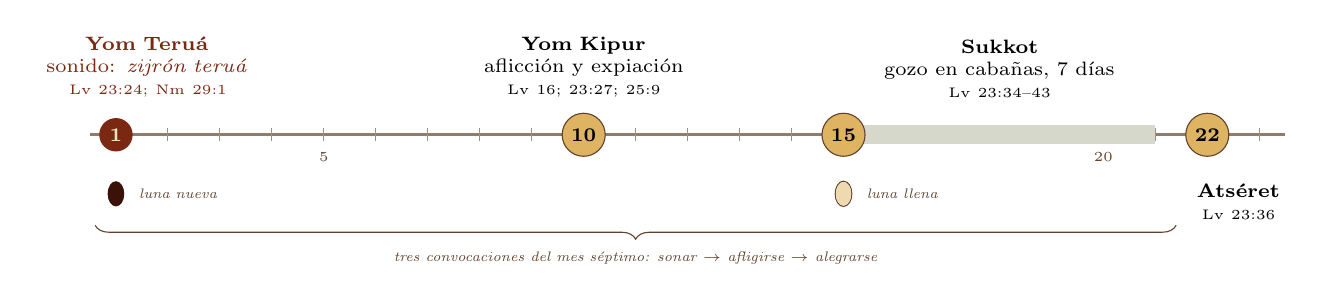
\begin{tikzpicture}[x=0.66cm,y=1cm,font=\scriptsize]
 \draw[line width=1pt,sepia!70] (0.5,0) -- (23.5,0);
 \foreach \d in {1,...,23}{\draw[sepia!60] (\d,-0.08) -- (\d,0.08);}
 \foreach \d in {5,20}{\node[below=3pt,font=\tiny,text=sepia] at (\d,0) {\d};}
 \fill[caferojizo] (1,-0.75) circle (0.16);
 \draw[sepia] (15,-0.75) circle (0.16); \fill[mostaza!40] (15,-0.75) circle (0.15);
 \node[right=3pt,font=\tiny\itshape,text=sepia] at (1.1,-0.75) {luna nueva};
 \node[right=3pt,font=\tiny\itshape,text=sepia] at (15.1,-0.75) {luna llena};
 \node[circle,fill=tierraroja,text=papiro,inner sep=2pt,font=\scriptsize\bfseries] (t) at (1,0) {1};
 \node[circle,fill=mostaza!80,draw=sepia,inner sep=2pt,font=\scriptsize\bfseries] (k) at (10,0) {10};
 \fill[oliva!25] (15,-0.12) rectangle (21,0.12);
 \node[circle,fill=mostaza!80,draw=sepia,inner sep=2pt,font=\scriptsize\bfseries] at (15,0) {15};
 \node[circle,fill=mostaza!80,draw=sepia,inner sep=2pt,font=\scriptsize\bfseries] at (22,0) {22};
 \node[above=10pt,text width=2.8cm,align=center,text=tierraroja] at (1.6,0) {\textbf{Yom Teruá}\\ sonido: \emph{zijrón teruá}\\ {\tiny Lv 23:24; Nm 29:1}};
 \node[above=10pt,text width=2.8cm,align=center] at (10,0) {\textbf{Yom Kipur}\\ aflicción y expiación\\ {\tiny Lv 16; 23:27; 25:9}};
 \node[above=10pt,text width=3.4cm,align=center] at (18,0) {\textbf{Sukkot}\\ gozo en cabañas, 7 días\\ {\tiny Lv 23:34--43}};
 \node[above=10pt,text width=1.6cm,align=center] at (22.6,-1.55) {\textbf{Atséret}\\ {\tiny Lv 23:36}};
 \draw[decorate,decoration={brace,amplitude=5pt,mirror},sepia] (0.6,-1.15) -- (21.4,-1.15) node[midway,below=6pt,font=\tiny\itshape,text=sepia] {tres convocaciones del mes séptimo: sonar $\rightarrow$ afligirse $\rightarrow$ alegrarse};
\end{tikzpicture}\par
{\footnotesize\color{sepia}\textit{Figura 2.} El mes séptimo como triple convocación. \textit{Nota.} Elaboración propia con Lv 23 y Nm 29. La secuencia de afectos (sonido, aflicción, gozo) es una síntesis del autor.}
\end{minipage}\end{center}

\subsection{El mes séptimo, el año sabático y el jubileo}
El mes séptimo es una pieza del ritmo del siete que ordena el tiempo de Israel. El séptimo día es \emph{shabat}; el séptimo mes concentra tres convocaciones; el séptimo año es \emph{shemitá}, en que la tierra descansa (Lv 25:1--7; Éx 23:10--11) y se remiten las deudas (Dt 15:1--2); y después de siete semanas de años llega el \emph{yovel}, el año cincuenta, en que cada uno vuelve a su posesión y a su familia (Lv 25:8--13). El sonido del mes séptimo enlaza esos niveles:

\hebverso{וְהַעֲבַרְתָּ שׁוֹפַר תְּרוּעָה בַּחֹדֶשׁ הַשְּׁבִעִי בֶּעָשׂוֹר לַחֹדֶשׁ \\ בְּיוֹם הַכִּפֻּרִים תַּעֲבִירוּ שׁוֹפָר בְּכָל־אַרְצְכֶם}
\begin{cita}Entonces harás tocar fuertemente la trompeta en el mes séptimo a los diez días del mes; el día de la expiación haréis tocar la trompeta por toda vuestra tierra. Y santificaréis el año cincuenta, y pregonaréis libertad en la tierra a todos sus moradores.\fuente{(Lv 25:9--10)}\end{cita}

El jubileo se anuncia el décimo día del mes, en Yom Kipur, y no el primero; pero se anuncia con la misma expresión, \emph{shofar teruá}, y en el mismo mes. El año sabático y el jubileo se cuentan, por tanto, desde el mes séptimo, como confirma la Misná al decir que el uno de Tishri es año nuevo ``para los años sabáticos y los jubileos'' (\emph{Rosh haShaná} 1:1). Deuteronomio añade el vínculo con la Palabra: ``al fin de cada siete años, en el año de la remisión, en la fiesta de los tabernáculos'', la ley debía leerse ante todo Israel (Dt 31:10--11). Nehemías 8 se parece a esa asamblea, porque la lectura comienza el primer día del mes séptimo y continúa ``cada día, desde el primer día hasta el último'' de la fiesta de los tabernáculos (Neh 8:18). La Figura~3 ordena los cuatro niveles.

\begin{center}\begin{minipage}{\linewidth}\centering
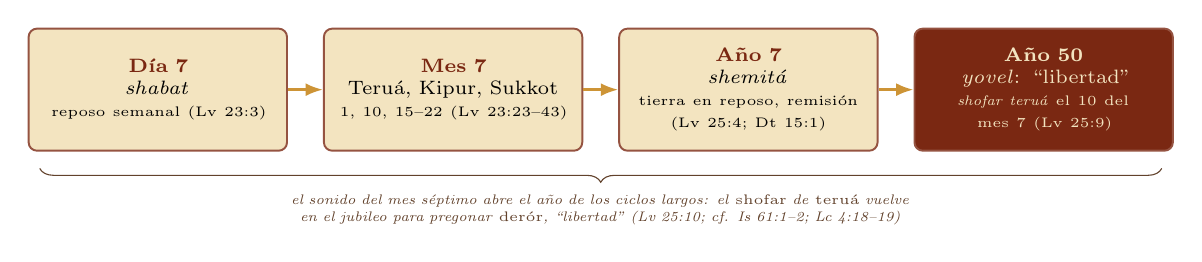
\begin{tikzpicture}[font=\scriptsize]
 \tikzset{n/.style={draw=tierraroja!80,line width=0.7pt,fill=papiro,rounded corners=3pt,text width=3.0cm,align=center,inner sep=4pt,minimum height=1.55cm}}
 \node[n] (a) at (0,0) {\textbf{\textcolor{tierraroja}{Día 7}}\\ \emph{shabat}\\ {\tiny reposo semanal (Lv 23:3)}};
 \node[n] (b) at (3.75,0) {\textbf{\textcolor{tierraroja}{Mes 7}}\\ Teruá, Kipur, Sukkot\\ {\tiny 1, 10, 15--22 (Lv 23:23--43)}};
 \node[n] (c) at (7.5,0) {\textbf{\textcolor{tierraroja}{Año 7}}\\ \emph{shemitá}\\ {\tiny tierra en reposo, remisión (Lv 25:4; Dt 15:1)}};
 \node[n,fill=tierraroja,text=papiro] (d) at (11.25,0) {\textbf{Año 50}\\ \emph{yovel}: ``libertad''\\ {\tiny \emph{shofar teruá} el 10 del mes 7 (Lv 25:9)}};
 \foreach \u/\v in {a/b,b/c,c/d}{\draw[-{Latex[length=2.2mm]},mostaza!90!tierraroja,line width=1pt] (\u)--(\v);}
 \draw[decorate,decoration={brace,amplitude=5pt,mirror},sepia] (-1.5,-1.0) -- (12.75,-1.0) node[midway,below=6pt,font=\tiny\itshape,text=sepia,text width=12cm,align=center] {el sonido del mes séptimo abre el año de los ciclos largos: el \emph{shofar} de \emph{teruá} vuelve en el jubileo para pregonar \emph{derór}, ``libertad'' (Lv 25:10; cf. Is 61:1--2; Lc 4:18--19)};
\end{tikzpicture}\par
{\footnotesize\color{sepia}\textit{Figura 3.} El ritmo del siete y el lugar del mes séptimo. \textit{Nota.} Elaboración propia con Lv 23; 25; Dt 15; 31.}
\end{minipage}\end{center}

Isaías recoge el lenguaje del jubileo cuando anuncia ``libertad'' (\heb{דְּרוֹר}, \emph{derór}, el término de Lv 25:10) a los cautivos y ``el año de la buena voluntad de \SENOR'' (Is 61:1--2), y Jesús lee ese texto en Nazaret como cumplido ``hoy'' (Lc 4:18--21). El vínculo de esa proclamación con el \emph{shofar} del mes séptimo es un eco posible y no una cita; aun así muestra que, ya dentro de la Torá, el sonido de este mes era el sonido de la liberación.

\subsection{Dos instrumentos: la trompeta de plata y el cuerno de carnero}
La palabra ``trompeta'' de las versiones españolas traduce dos instrumentos distintos. La \heb{חֲצֹצְרָה} (\emph{jatsotsrá}) es una trompeta recta de metal, fabricada por orden divina en plata batida (\emph{miqshá}, Nm 10:2) y tocada en pares por los sacerdotes. Josefo la describe como un tubo estrecho de poco menos de un codo que se ensancha en campana (\emph{Ant.} 3.12.6), y el Arco de Tito, en Roma, muestra dos de ellas entre los despojos del templo. El \heb{שׁוֹפָר} (\emph{shofar}) es un cuerno de animal, de carnero en la mayoría de los textos, sin fabricación metálica, capaz de pocos sonidos y de timbre áspero. Lo tocan sacerdotes en Jericó, pero también un caudillo como Aod (Jue 3:27), Gedeón y sus trescientos (Jue 7:16--22) o un rebelde como Seba (2~S 20:1). La Tabla~2 y la Figura~4 comparan ambos.

\begin{center}\begin{minipage}{\linewidth}\centering\small\renewcommand{\arraystretch}{1.18}
\begin{tabular}{@{}L{2.4cm}L{6.0cm}L{6.0cm}@{}}
\toprule
& \textbf{\heb{חֲצֹצְרָה} \emph{jatsotsrá}} & \textbf{\heb{שׁוֹפָר} \emph{shofar}} \\ \midrule
Material & plata batida, \emph{miqshá} (Nm 10:2) & cuerno natural; \emph{qéren hayovel}, ``cuerno de carnero'' (Jos 6:5) \\
Origen & hecha por mandato en el desierto & instrumento pastoral, previo a la ley \\
Quién la toca & los hijos de Aarón, ``estatuto perpetuo'' (Nm 10:8) & sacerdotes (Jos 6), jueces, el pueblo, el centinela (Ez 33:3) \\
Usos & convocar, partir, guerra, fiestas y lunas nuevas sobre los holocaustos (Nm 10); dedicación del templo (2~Cr 5:12) & teofanía del Sinaí (Éx 19:16, 19), Jericó (Jos 6), coronación (1~R 1:34), jubileo (Lv 25:9), alarma profética (Jl 2:1; Os 5:8) \\
LXX & \grc{σάλπιγξ} & \grc{σάλπιγξ}; a veces \grc{κερατίνη} (Sal 97:6 LXX [98:6]) \\
Sonido & \emph{tekiá} (toque largo) y \emph{teruá} (toque de alarma) (Nm 10:5--7) & \emph{teruá}; ``sonido prolongado'' (\emph{bimshoj}, Éx 19:13; Jos 6:5) \\
\bottomrule
\end{tabular}\par
{\footnotesize\color{sepia}\textit{Tabla 2.} Las dos ``trompetas'' de la Biblia hebrea. \textit{Nota.} Elaboración propia con la BHS, la LXX y de Vaux (1985).}
\end{minipage}\end{center}

\begin{center}\begin{minipage}{\linewidth}\centering
\begin{tikzpicture}[font=\scriptsize]
 \node[draw=tierraroja,line width=0.8pt,fill=papiro,rounded corners=3pt,text width=4.6cm,inner sep=6pt] (j) at (0,0) {\centering\textbf{\textcolor{tierraroja}{Jatsotsrá}} \heb{חֲצֹצְרָה}\par\RaggedRight
   plata, en par, sacerdotal\\ $\bullet$ convocar (dos) / príncipes (una)\\ $\bullet$ partir los campamentos\\ $\bullet$ guerra: ``seréis recordados''\\ $\bullet$ fiestas y lunas nuevas: ``por memoria''\\ {\tiny\color{sepia} Nm 10:1--10; 31:6; 2 Cr 5:12; 13:12}};
 \node[draw=tierraroja,line width=0.8pt,fill=papiro,rounded corners=3pt,text width=4.6cm,inner sep=6pt] (s) at (9,0) {\centering\textbf{\textcolor{tierraroja}{Shofar}} \heb{שׁוֹפָר}\par\RaggedRight
   cuerno de carnero, natural\\ $\bullet$ teofanía: Sinaí\\ $\bullet$ guerra santa: Jericó, Gedeón\\ $\bullet$ coronación del rey\\ $\bullet$ jubileo: ``libertad''\\ {\tiny\color{sepia} Éx 19; Jos 6; Jue 7; 1 R 1:34; Lv 25:9}};
 \node[ellipse,draw=mostaza!90!tierraroja,line width=1.2pt,fill=mostaza!25,inner sep=3pt,text width=2.4cm,align=center] (t) at (4.5,0) {\textbf{teruá} \heb{תְּרוּעָה}\\ el sonido común\\ {\tiny Lv 23:24; Nm 29:1}};
 \draw[-{Latex[length=2.5mm]},mostaza!90!tierraroja,line width=1pt] (j) -- (t);
 \draw[-{Latex[length=2.5mm]},mostaza!90!tierraroja,line width=1pt] (s) -- (t);
 \node[text width=12cm,align=center,font=\tiny\itshape,text=sepia] at (4.5,-2.0) {Sal 98:6 une los dos: ``Aclamad (\emph{hariú}) con trompetas (\emph{jatsotsrot}) y sonido de bocina (\emph{shofar}) delante del rey \SENOR''. Lv 23:24 nombra el sonido, no el instrumento.};
\end{tikzpicture}\par
{\footnotesize\color{sepia}\textit{Figura 4.} Jatsotsrá y shofar: dos instrumentos, un mismo sonido. \textit{Nota.} Elaboración propia con la BHS.}
\end{minipage}\end{center}

\subsection{El Sinaí: el primer shofar}
El primer \emph{shofar} de la Biblia no lo toca un hombre. Al tercer día, en el Sinaí, ``vinieron truenos y relámpagos, y espesa nube sobre el monte, y sonido de bocina muy fuerte; y se estremeció todo el pueblo'' (Éx 19:16). El sonido crece mientras Dios habla: ``El sonido de la bocina iba aumentando en extremo; Moisés hablaba, y Dios le respondía con voz tronante'' (19:19). La orden previa ya lo había vinculado con el acceso a Dios, pues ``cuando suene largamente la bocina (\heb{בִּמְשֹׁךְ הַיֹּבֵל}), subirán al monte'' (19:13). El \emph{shofar} del Sinaí es, pues, teofánico: anuncia la presencia de Dios y convoca al pueblo a su encuentro (Éx 19:17; 20:18). Hebreos lo recuerda entre los rasgos del monte que no se puede tocar, ``el sonido de la trompeta, y la voz que hablaba'' (He 12:19).

\subsection{Jericó: la trompeta y la caída de los muros}
El segundo gran \emph{shofar} es el de Jericó, el hito que la serie vincula con esta fiesta. Josué 6 narra una guerra que no se pelea; Dios da la orden:

\hebverso{וְשִׁבְעָה כֹהֲנִים יִשְׂאוּ שִׁבְעָה שׁוֹפְרוֹת הַיּוֹבְלִים לִפְנֵי הָאָרוֹן \\ וּבַיּוֹם הַשְּׁבִיעִי תָּסֹבּוּ אֶת־הָעִיר שֶׁבַע פְּעָמִים וְהַכֹּהֲנִים יִתְקְעוּ בַּשּׁוֹפָרוֹת}
\begin{cita}Y siete sacerdotes llevarán siete bocinas de cuernos de carnero delante del arca; y al séptimo día daréis siete vueltas a la ciudad, y los sacerdotes tocarán las bocinas. Y cuando toquen prolongadamente el cuerno de carnero, así que oigáis el sonido de la bocina, todo el pueblo gritará a gran voz, y el muro de la ciudad caerá; entonces subirá el pueblo, cada uno derecho hacia adelante.\fuente{(Jos 6:4--5)}\end{cita}

La ejecución sigue la orden con precisión ritual. Durante seis días se da una vuelta diaria, con el pueblo en silencio y el \emph{shofar} de los sacerdotes sonando sin cesar (6:9, 13); el séptimo día se dan siete vueltas, y a la séptima Josué ordena: ``Gritad, porque \SENOR{} os ha entregado la ciudad'' (6:16). Entonces ``el pueblo gritó, y los sacerdotes tocaron las bocinas; y aconteció que cuando el pueblo hubo oído el sonido de la bocina, gritó con gran vocerío, y el muro se derrumbó'' (6:20). Ese ``gran vocerío'' es \heb{תְּרוּעָה גְדוֹלָה} (\emph{teruá gedolá}), la misma palabra de Lv 23:24 y Nm 29:1; en Jericó la \emph{teruá} es a la vez el toque de los sacerdotes y el grito del pueblo.

\begin{center}\begin{minipage}{\linewidth}\centering
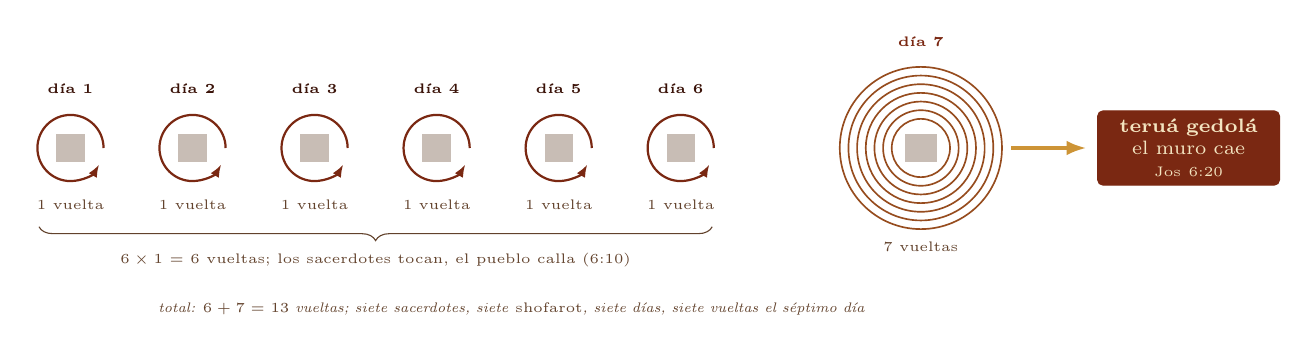
\begin{tikzpicture}[font=\scriptsize]
 \foreach \d in {1,...,6}{
   \pgfmathsetmacro{\x}{(\d-1)*1.55}
   \fill[sepia!35] (\x-0.18,-0.18) rectangle (\x+0.18,0.18);
   \draw[tierraroja,line width=0.8pt,-{Latex[length=1.6mm]}] (\x,0) ++(0:0.42) arc (0:330:0.42);
   \node[font=\tiny\bfseries,text=caferojizo] at (\x,0.75) {día \d};
   \node[font=\tiny,text=sepia] at (\x,-0.72) {1 vuelta};}
 \fill[sepia!35] (10.6,-0.18) rectangle (11.0,0.18);
 \foreach \r in {1,...,7}{\draw[tierraroja!70!mostaza,line width=0.6pt] (10.8,0) circle ({0.26+0.11*\r});}
 \node[font=\tiny\bfseries,text=tierraroja] at (10.8,1.35) {día 7};
 \node[font=\tiny,text=sepia] at (10.8,-1.25) {7 vueltas};
 \draw[-{Latex[length=2.5mm]},mostaza!90!tierraroja,line width=1.2pt] (11.95,0) -- (12.9,0);
 \node[draw=tierraroja,fill=tierraroja,text=papiro,rounded corners=2pt,text width=2.1cm,align=center,inner sep=3pt] at (14.2,0) {\textbf{teruá gedolá}\\ el muro cae\\ {\tiny Jos 6:20}};
 \draw[decorate,decoration={brace,amplitude=5pt,mirror},sepia] (-0.4,-1.0) -- (8.15,-1.0) node[midway,below=6pt,font=\tiny,text=sepia] {$6\times1$ = 6 vueltas; los sacerdotes tocan, el pueblo calla (6:10)};
 \node[font=\tiny\itshape,text=sepia] at (5.6,-2.05) {total: $6 + 7 = 13$ vueltas; siete sacerdotes, siete \emph{shofarot}, siete días, siete vueltas el séptimo día};
\end{tikzpicture}\par
{\footnotesize\color{sepia}\textit{Figura 5.} Jericó: seis días con una vuelta y un séptimo día con siete. \textit{Nota.} Elaboración propia con Jos 6:3--20.}
\end{minipage}\end{center}

\begin{nota}[Precisión: Jericó y el calendario]
Levítico 23 no menciona Jericó, y el libro de Josué no fecha la caída de la ciudad el primer día del mes séptimo. Según la cronología del propio libro, Israel cruzó el Jordán ``el día diez del mes primero'' (Jos 4:19), celebró la Pascua en Gilgal el día catorce (5:10) y luego rodeó Jericó; la caída ocurrió, por tanto, en primavera, pocos días después de Pésaj. El vínculo entre la fiesta y Jericó que propone la serie es temático y tipológico (el sonido del \emph{shofar}, la \emph{teruá} del pueblo, el número siete, la entrada en la heredad), no calendárico. Así lo expongo en la §7.
\end{nota}

\subsection{La fiesta en la historia narrada de Israel}
La historia de Israel menciona el mes séptimo en momentos de fundación. Salomón reúne a Israel para subir el arca del pacto al templo ``en el mes de Etanim, que es el mes séptimo, en el día de la fiesta solemne'' (1~R 8:1--2), un hecho que ya destaqué en mi presentación sobre la fiesta, y el cronista añade que ciento veinte sacerdotes tocaban trompetas cuando la gloria llenó la casa (2~Cr 5:12--14). Después del exilio, el altar se levanta antes que el templo, y el culto se reanuda ``desde el primer día del mes séptimo'' (Esd 3:6). Bajo Nehemías, ese primer día del mes séptimo se convierte en día de la Palabra: Esdras lee ``desde el alba hasta el mediodía'' (Neh 8:3), los levitas ``ponían el sentido'' (8:8), y el llanto del pueblo se convierte, por orden de sus líderes, en banquete compartido con ``los que no tienen nada preparado'' (8:10--12).

Nehemías 8 merece una palabra más. El texto no menciona trompetas, pero el día es reconocible por la fecha y por su carácter de asamblea santa. El pueblo llora porque la ley le revela su distancia de Dios, y los líderes lo corrigen: ``el día es santo'', y el gozo de \SENOR{} es su ``fuerza'' (\heb{מָעֻזְּכֶם}, \emph{ma'uzjem}, su refugio fortificado). Diez días antes de Yom Kipur, el texto ya une los dos polos que la tradición posterior desarrollará en este día, la conciencia de pecado y la alegría de la convocación.

\subsection{En el Segundo Templo}
Las fuentes del Segundo Templo muestran que la fiesta se celebraba y que se buscaba su sentido. Todas son posteriores al Antiguo Testamento y las cito como testimonio de su interpretación.

\begin{itemize}\setlength{\itemsep}{2pt}
\item \textbf{Jubileos} (s.~II a.\,e.\,c.) hace del primer día de los meses primero, cuarto, séptimo y décimo ``días de memoria'' instituidos por Noé (Jub 6:23--29).
\item \textbf{Qumrán}: el Rollo del Templo regula las ofrendas del primer día del mes séptimo como ``día de memoria'' (11Q19 25), y el Rollo de la Guerra prescribe trompetas con inscripciones para cada maniobra de la batalla final (1QM 2--3), una relectura escatológica de Nm 10 (García Martínez, 1992).
\item \textbf{Filón de Alejandría} llama a la fiesta ``de las trompetas'' y le da dos sentidos: memoria de la ley dada en el Sinaí al son de trompeta, y figura de Dios que pone fin a la guerra y da la paz (\emph{De specialibus legibus} 2.188--192).
\item \textbf{Josefo} registra los sacrificios del primer día del mes séptimo, que los macedonios llaman \emph{Hiperbereteo} (\emph{Ant.} 3.10.2).
\item \textbf{La Misná} (ca.~200 e.\,c.) describe la práctica del templo: el \emph{shofar} en el centro y dos trompetas a los lados; ``el \emph{shofar} prolonga y las trompetas acortan, porque el precepto del día es el \emph{shofar}'' (\emph{Rosh haShaná} 3:3).
\end{itemize}

La Figura~6 ordena estos testimonios junto con los hitos bíblicos.

\begin{center}\begin{minipage}{\linewidth}\centering
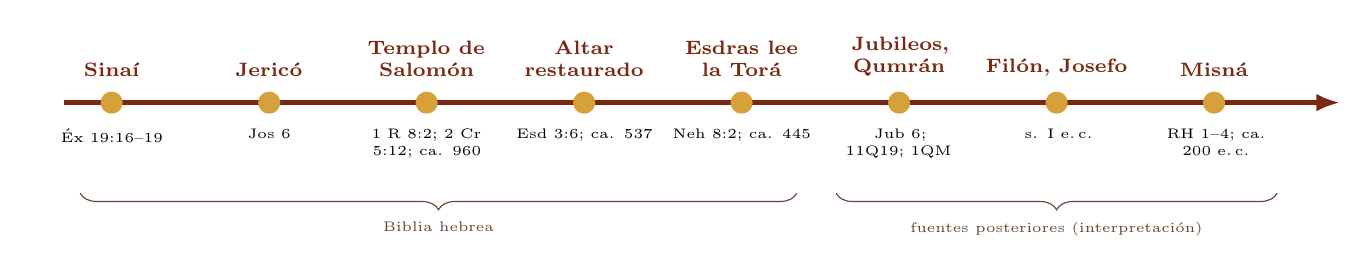
\begin{tikzpicture}[font=\scriptsize]
 \draw[line width=1.6pt,tierraroja,-{Latex[length=3mm]}] (0,0) -- (16.2,0);
 \foreach \x/\a/\b in {0.6/{Sinaí}/{Éx 19:16--19}, 2.6/{Jericó}/{Jos 6}, 4.6/{Templo de Salomón}/{1 R 8:2; 2 Cr 5:12; ca. 960}, 6.6/{Altar restaurado}/{Esd 3:6; ca. 537}, 8.6/{Esdras lee la Torá}/{Neh 8:2; ca. 445}, 10.6/{Jubileos, Qumrán}/{Jub 6; 11Q19; 1QM}, 12.6/{Filón, Josefo}/{s. I e.\,c.}, 14.6/{Misná}/{RH 1--4; ca. 200 e.\,c.}}{
   \fill[mostaza] (\x,0) circle (4pt);
   \node[above=6pt,font=\scriptsize\bfseries,text=tierraroja,text width=1.9cm,align=center] at (\x,0) {\a};
   \node[below=6pt,text width=1.85cm,align=center,font=\tiny] at (\x,0) {\b};}
 \draw[decorate,decoration={brace,amplitude=6pt,mirror},sepia] (0.2,-1.15) -- (9.3,-1.15) node[midway,below=7pt,font=\tiny,text=sepia] {Biblia hebrea};
 \draw[decorate,decoration={brace,amplitude=6pt,mirror},sepia] (9.8,-1.15) -- (15.4,-1.15) node[midway,below=7pt,font=\tiny,text=sepia] {fuentes posteriores (interpretación)};
\end{tikzpicture}\par
{\footnotesize\color{sepia}\textit{Figura 6.} La trompeta del mes séptimo en la historia. \textit{Nota.} Elaboración propia. Fechas aproximadas a.\,e.\,c. salvo indicación; el Sinaí y Jericó dependen de la cronología del éxodo (ca.~1446 o ca.~1260 a.\,e.\,c.; la serie propone 1529/1530).}
\end{minipage}\end{center}

%===================================================================
\section{Lectura filológica}

El vocabulario de la fiesta es pequeño y preciso. Hay un sonido (\emph{teruá}), dos instrumentos (\emph{shofar}, \emph{jatsotsrá}) con un calificativo (\emph{yovel}), un verbo de tocar (\emph{taqa'}), una raíz de memoria (\emph{zajar}), una palabra de reposo (\emph{shabatón}) y una palabra discutida del calendario (\emph{kese}).

\begin{filologia}[\heb{תְּרוּעָה} \emph{teruá}]
Sustantivo de la raíz \heb{ר־ו־ע} (\emph{r-w-'}), cuyo verbo en hifil, \heb{הֵרִיעַ} (\emph{heria'}), significa ``gritar, dar voces, tocar alarma''. Su campo cubre cuatro situaciones: el \textbf{grito de guerra} y la alarma (Nm 10:5, 9; Jos 6:5, 20; Jer 4:19; Am 1:14); la \textbf{aclamación al rey}, humano o divino (Nm 23:21, ``júbilo de rey en él''; 1~S 10:24); el \textbf{júbilo del culto} (2~S 6:15; Esd 3:11; Sal 47:5 [47:6], ``Subió Dios con júbilo, \SENOR{} con sonido de trompeta''); y el grito que hace temblar la tierra cuando llega el arca: ``todo Israel gritó con tan gran júbilo que la tierra tembló'' (1~S 4:5--6). El Salmo 89:15 [89:16] la convierte en conocimiento: \heb{אַשְׁרֵי הָעָם יֹדְעֵי תְרוּעָה}, ``Bienaventurado el pueblo que sabe aclamarte'', literalmente ``que conoce la \emph{teruá}''. Strong (H8643) resume el abanico: clamor, aclamación de alegría, grito de batalla, clarinada, alarma, júbilo. Puede ser voz humana o sonido de instrumento; en Lv 23:24 no se especifica.
\end{filologia}

\begin{filologia}[\heb{שׁוֹפָר} \emph{shofar} y \heb{יוֹבֵל} \emph{yovel}]
\emph{Shofar} es el cuerno usado como instrumento. Sale 72 veces en 63 versículos de la Biblia hebrea (conteo propio del lema, Strong H7782, sobre el Códice de Leningrado). La Misná admite cualquier cuerno salvo el de vaca, porque se llama \emph{qéren}, no \emph{shofar} (\emph{Rosh haShaná} 3:2). \emph{Yovel} califica al cuerno en Éx 19:13 y Jos 6:4--13 (\heb{שׁוֹפְרוֹת הַיּוֹבְלִים}, ``cuernos de carnero''; \heb{קֶרֶן הַיּוֹבֵל}, Jos 6:5). El Talmud recuerda que Rabí Aquiba oyó en Arabia \emph{yuvla} por ``carnero'' (b.~\emph{Rosh haShaná} 26a). De ahí el nombre del año del jubileo (Lv 25:10), anunciado con \emph{shofar teruá} (25:9): el año del ``cuerno''.
\end{filologia}

\begin{filologia}[\heb{חֲצֹצְרָה} \emph{jatsotsrá}]
Trompeta recta de metal (Nm 10:2; 31:6; 2~R 11:14; 2~Cr 5:12--13). La forma, con reduplicación de consonantes, se ha explicado como onomatopéyica (hipótesis). Casi siempre aparece en plural y en manos de sacerdotes, y es el instrumento propio del culto del templo en Crónicas (1~Cr 15:24; 16:6; 2~Cr 29:26--28). La LXX la traduce \grc{σάλπιγξ}.
\end{filologia}

\begin{filologia}[\heb{מִקְרָא} \emph{mikrá}]
Sustantivo de \heb{קָרָא} (\emph{qará}, ``llamar, proclamar, leer''). En Lv 23:2, 4 las fiestas son \heb{מִקְרָאֵי קֹדֶשׁ}, ``convocaciones santas''. Los léxicos registran tres sentidos: la \textbf{convocación} o asamblea (Lv 23; Nm 28--29), el \textbf{llamado} (Nm 10:2, ``para convocar la congregación'') y la \textbf{lectura} pública: ``y ponían el sentido, de modo que entendiesen la lectura'' (\heb{בַּמִּקְרָא}, Neh 8:8), precisamente el primer día del mes séptimo (BDB; HALOT). La concordancia de Strong (H4744) añade la glosa inglesa \emph{rehearsal}, que en su época significaba ``recitación'', y de ahí la lectura que propuse en mi presentación: las solemnidades como ``ensayo'' de lo que vendrá. Esa lectura es una analogía fecunda, y debe presentarse como tal: el término dice ``convocación'' y ``lectura''; la idea de que la fiesta anticipa un cumplimiento procede de Col 2:16--17 (``sombra de lo por venir''), no del sustantivo.
\end{filologia}

\begin{filologia}[\heb{תָּקַע} \emph{taqa'}]
``Clavar, hincar'' (una estaca, Jue 4:21; una tienda, Gn 31:25), ``batir palmas'' (Sal 47:1 [47:2]) y ``tocar'' un instrumento de viento: \heb{תִּקְעוּ שׁוֹפָר}, ``tocad trompeta'' (Jl 2:1, 15; Sal 81:3 [81:4]). Nm 10:7 distingue \emph{taqa'} sin \emph{heria'}: ``tocaréis, mas no con sonido de alarma''. De ahí la terminología posterior: \emph{tekiá} (\heb{תְּקִיעָה}), el toque sostenido, frente a \emph{teruá}, el toque quebrado.
\end{filologia}

\begin{filologia}[\heb{זִכָּרוֹן} \emph{zikarón} / \heb{זָכַר} \emph{zajar}]
\emph{Zajar} es más que traer algo a la mente; es recordar para actuar. Cuando el sujeto es Dios, el verbo marca el giro de la historia: ``Y se acordó Dios de Noé'' (\heb{וַיִּזְכֹּר אֱלֹהִים אֶת־נֹחַ}, Gn 8:1), y las aguas bajan; ``oyó Dios el gemido de ellos, y se acordó de su pacto'' (Éx 2:24), y comienza el éxodo; ``\SENOR{} se acordó de ella'' (1~S 1:19), y Ana concibe. El sustantivo \emph{zikarón} designa lo que se pone ``delante de \SENOR'' para memoria: las piedras del efod (Éx 28:12, 29), la plata de las expiaciones (Éx 30:16), las trompetas (Nm 10:10). Pero también la memoria del pueblo: Pésaj ``os será en memoria'' (Éx 12:14). \emph{Zijrón teruá} admite ambos sentidos; Nm 10:9--10 privilegia el primero.
\end{filologia}

\begin{filologia}[\heb{שַׁבָּתוֹן} \emph{shabatón} y \heb{כֵּסֶה} \emph{kese}]
\emph{Shabatón}, con sufijo abstracto \emph{-on}, es ``reposo solemne''. Se dice del sábado (\emph{shabat shabatón}, Éx 31:15; Lv 23:3), de Yom Kipur (Lv 16:31; 23:32), del año sabático (Lv 25:4) y, solo como \emph{shabatón}, de Yom Teruá y del primer y octavo día de Sukkot (Lv 23:24, 39). La RVR1960 traduce ``día de reposo''. \emph{Kese} (\heb{כֵּסֶה}) aparece en Sal 81:3 [81:4], y con \emph{álef} (\heb{כֵּסֶא}) en Pr 7:20, ``el día señalado''. Una lectura lo relaciona con el siríaco \emph{kes'a} y el acadio \emph{kusê}, ``luna llena''; la tradición rabínica lo relaciona con \emph{kasá}, ``cubrir'': la fiesta en que la luna está cubierta, es decir, la luna nueva (b.~\emph{Rosh haShaná} 8a--b). Véase §5.3.
\end{filologia}

\begin{filologia}[Septuaginta: \grc{σάλπιγξ}, \grc{μνημόσυνον}, \grc{σημασία}]
La LXX traduce \emph{zijrón teruá} como \grc{μνημόσυνον σαλπίγγων}, ``memorial de trompetas'' (Lv 23:24), y así introduce el instrumento que el hebreo no nombra. El \emph{shabatón} es \grc{ἀνάπαυσις} y el \emph{mikrá kódesh}, \grc{κλητὴ ἁγία}, ``llamada santa''. En Nm 29:1, \emph{yom teruá} se vuelve \grc{ἡμέρα σημασίας}, ``día de señal'', un término técnico para la señal militar. En los Salmos, \emph{teruá} se traduce \grc{ἀλαλαγμός}, ``grito de júbilo'' (Sal 46:6 LXX [47:6]; 88:16 LXX [89:16]). El \emph{kese} de Sal 81:4 se vuelve \grc{ἐν εὐσήμῳ ἡμέρᾳ}, ``en el día bien señalado'' (Sal 80:4 LXX).
\end{filologia}

\begin{filologia}[Nuevo Testamento: \grc{σάλπιγξ}, \grc{φωνή}, \grc{κέλευσμα}]
\grc{Σάλπιγξ} (``trompeta'') y \grc{σαλπίζω} (``tocar trompeta'') aparecen en el NT sobre todo en contextos escatológicos: Mt 24:31 (\grc{μετὰ σάλπιγγος μεγάλης}); 1~Co 15:52 (\grc{ἐν τῇ ἐσχάτῃ σάλπιγγι· σαλπίσει γάρ}); 1~Ts 4:16 (\grc{ἐν σάλπιγγι θεοῦ}); Ap 1:10 y 4:1 (``una voz como de trompeta''); Ap 8--11 (siete trompetas). \grc{Φωνή} (``voz, sonido'') sirve para la voz de la trompeta (\grc{σάλπιγγος ἤχῳ καὶ φωνῇ ῥημάτων}, He 12:19) y para la voz humana. \grc{Κέλευσμα} (1~Ts 4:16, \emph{hápax} del NT) es la voz de mando: la orden del capitán a la tropa o del cómitre a los remeros (BDAG). La RVR1960 traduce ``voz de mando''.
\end{filologia}

La Figura~7 muestra el campo semántico de \emph{teruá}; la Figura~8, el paso de la palabra del hebreo a la Septuaginta, al Nuevo Testamento y al español.

\begin{center}\begin{minipage}{\linewidth}\centering
\begin{tikzpicture}[font=\scriptsize]
 \node[ellipse,draw=tierraroja,line width=1.2pt,fill=tierraroja!10,inner sep=4pt,align=center] (c) at (0,0) {\large\heb{תְּרוּעָה}\\ \textbf{teruá}\\ {\tiny raíz \heb{רוע}}};
 \node (a) at (-4.6,1.4) [draw=tierraroja!70,fill=papiro,rounded corners=3pt,inner sep=4pt,text width=3.6cm] {\textbf{\textcolor{tierraroja}{Alarma}}\\ partir el campamento, peligro\\ {\tiny\color{sepia}Nm 10:5--6, 9; Jer 4:19; Os 5:8}};
 \node (g) at (4.6,1.4) [draw=tierraroja!70,fill=papiro,rounded corners=3pt,inner sep=4pt,text width=3.6cm] {\textbf{\textcolor{tierraroja}{Guerra}}\\ grito de combate, victoria\\ {\tiny\color{sepia}Jos 6:5, 20; 1 S 17:20; 2 Cr 13:12--15}};
 \node (j) at (-4.6,-1.4) [draw=tierraroja!70,fill=papiro,rounded corners=3pt,inner sep=4pt,text width=3.6cm] {\textbf{\textcolor{tierraroja}{Júbilo y realeza}}\\ aclamación al Rey, culto\\ {\tiny\color{sepia}Nm 23:21; 1 S 4:5; Sal 47:5; 89:15; Esd 3:11}};
 \node (m) at (4.6,-1.4) [draw=tierraroja!70,fill=papiro,rounded corners=3pt,inner sep=4pt,text width=3.6cm] {\textbf{\textcolor{tierraroja}{Memoria ante Dios}}\\ ``seréis recordados''\\ {\tiny\color{sepia}Nm 10:9--10; Lv 23:24; Nm 29:1}};
 \foreach \n in {a,g,j,m}{\draw[-{Latex[length=2.2mm]},mostaza!90!tierraroja,line width=1pt] (c) -- (\n);}
\end{tikzpicture}\par
{\footnotesize\color{sepia}\textit{Figura 7.} El campo semántico de \emph{teruá}. \textit{Nota.} Elaboración propia con la BHS y BDB (Brown et al., 1906).}
\end{minipage}\end{center}

\begin{center}\begin{minipage}{\linewidth}\centering
\begin{tikzpicture}[font=\scriptsize,node distance=0.55cm]
 \node[draw=tierraroja,line width=0.8pt,fill=papiro,rounded corners=3pt,text width=3.2cm,align=center,inner sep=5pt] (h) {\textbf{Hebreo}\\ \heb{זִכְרוֹן תְּרוּעָה} (Lv 23:24)\\ \heb{יוֹם תְּרוּעָה} (Nm 29:1)\\ \heb{שׁוֹפָר}, \heb{חֲצֹצְרָה}};
 \node[draw=tierraroja,line width=0.8pt,fill=papiro,rounded corners=3pt,text width=3.2cm,align=center,inner sep=5pt,right=of h] (l) {\textbf{Septuaginta}\\ \grc{μνημόσυνον σαλπίγγων}\\ \grc{ἡμέρα σημασίας}\\ \grc{σάλπιγξ}, \grc{ἀλαλαγμός}};
 \node[draw=mostaza,line width=1.4pt,fill=tierraroja,text=papiro,rounded corners=3pt,text width=3.2cm,align=center,inner sep=5pt,right=of l] (n) {\textbf{Nuevo Testamento}\\ \grc{ἐσχάτῃ σάλπιγγι} (1 Co 15:52)\\ \grc{σάλπιγγι θεοῦ} (1 Ts 4:16)\\ \grc{ἐσάλπισεν} (Ap 11:15)};
 \node[draw=tierraroja,line width=0.8pt,fill=papiro,rounded corners=3pt,text width=3.2cm,align=center,inner sep=5pt,right=of n] (e) {\textbf{RVR1960}\\ ``conmemoración al son de trompetas''\\ ``día de sonar las trompetas''\\ ``la final trompeta''};
 \draw[-{Latex[length=2.5mm]},mostaza!90!tierraroja,line width=1.2pt] (h)--(l);
 \draw[-{Latex[length=2.5mm]},mostaza!90!tierraroja,line width=1.2pt] (l)--(n);
 \draw[-{Latex[length=2.5mm]},mostaza!90!tierraroja,line width=1.2pt] (n)--(e);
 \node[below=0.35cm of l.south east,text width=13cm,align=center,font=\tiny\itshape,text=sepia,anchor=north] {la LXX convierte el ``sonido'' en ``trompetas'' y la ``memoria'' en ``memorial''; el NT hereda la trompeta como señal de Dios en el fin};
\end{tikzpicture}\par
{\footnotesize\color{sepia}\textit{Figura 8.} De \emph{zijrón teruá} a ``la final trompeta''. \textit{Nota.} Elaboración propia con la BHS, la LXX (Rahlfs-Hanhart, 2006) y NA28.}
\end{minipage}\end{center}

%===================================================================
\section{Lectura textual: instrumento, salmo, año nuevo y fecha}

\subsection{¿Qué instrumento supone Levítico 23?}
El texto masorético de Lv 23:24 y Nm 29:1 no nombra el instrumento, y la respuesta depende de con qué texto se lea. Con Nm 10:10, que manda tocar las \emph{jatsotsrot} ``en vuestras solemnidades, y en los principios de vuestros meses'', la fiesta del primero del mes séptimo es una luna nueva solemne con trompetas de plata. Con Sal 81:3 [81:4] y Lv 25:9, el instrumento es el \emph{shofar}. La Misná combina ambos en el templo y da la primacía al \emph{shofar} (\emph{Rosh haShaná} 3:3--4). La Septuaginta, al traducir ``memorial de trompetas'', no decide, porque usa \grc{σάλπιγξ} para los dos. El Targum Onqelos, por su parte, traduce \emph{teruá} por \heb{יַבָּבָא} (\emph{yabava}), ``sollozo, lamento'', la palabra con que el Talmud identifica el sonido quebrado del \emph{shofar} con el gemido de la madre de Sísara (Jue 5:28; b.~\emph{Rosh haShaná} 33b).

\subsection{``Año nuevo'': la expresión y la cosa}
El nombre \heb{רֹאשׁ הַשָּׁנָה} (\emph{rosh hashaná}) aparece una sola vez en la Biblia, en Ez 40:1, ``en el principio del año, a los diez días del mes'', y ahí no designa esta fiesta. Quien fija el uso es la Misná: ``Hay cuatro años nuevos: el uno de Nisán es año nuevo para los reyes y las fiestas; el uno de Elul, para el diezmo del ganado; el uno de Tishri, para los años, los años sabáticos y los jubileos, la plantación y las hortalizas; el uno de Shevat, para el árbol'' (\emph{Rosh haShaná} 1:1, trad. propia). Que el uno de Tishri sea año nuevo para el cómputo de años, el \emph{shemitá} y el \emph{yovel} coincide con la ley, donde el jubileo empieza en el mes séptimo (Lv 25:9) y la lectura de la ley del año sabático se hace en Sukkot (Dt 31:10--11).

\begin{nota}[Precisión textual]
\textbf{1.} La Biblia no llama a esta fiesta ``año nuevo'' ni ``Rosh haShaná''; la llama \emph{zijrón teruá} y \emph{yom teruá}. ``Rosh haShaná'' como nombre de la fiesta es uso de la Misná. \textbf{2.} Éx 12:2 pone el principio de los meses en primavera; Éx 23:16 y 34:22 suponen un año agrícola que gira en otoño. Las dos cuentas conviven en la Biblia. \textbf{3.} El TM de Lv 23:24 dice \emph{zijrón teruá}; la LXX añade el instrumento (\grc{σαλπίγγων}) y el Targum Onqelos interpreta el sonido como lamento (\emph{yabava}). Este capítulo sigue el TM y la RVR1960, que con la LXX traduce ``al son de trompetas''.
\end{nota}

\subsection{Salmo 81:3 [81:4]: ¿luna nueva o luna llena?}
\hebverso{תִּקְעוּ בַחֹדֶשׁ שׁוֹפָר בַּכֵּסֶה לְיוֹם חַגֵּנוּ}
\begin{cita}Tocad la trompeta en la nueva luna, en el día señalado, en el día de nuestra fiesta solemne. Porque estatuto es de Israel, ordenanza del Dios de Jacob.\fuente{(Sal 81:3--4 [81:4--5])}\end{cita}

El versículo tiene dos datos de tiempo, \emph{bajódesh} (``en el mes'' o ``en la luna nueva'') y \emph{bakese}, y una designación de fiesta, \emph{jag}, que en la Biblia suele aplicarse a las tres fiestas de peregrinación (Pésaj/Matsot, Shavuot, Sukkot) y no a la luna nueva. Si \emph{kese} es ``luna llena'' (siríaco \emph{kes'a}; acadio \emph{kusê}), el salmo hablaría de Sukkot, el día quince, o quizá de Pésaj, ya que el v.~5 [6] menciona la salida de Egipto; el toque iría de la luna nueva a la luna llena, lectura que discuten los comentarios modernos (p.~ej., Tate, 1990). Si \emph{kese} es ``cubierta'', como lee el Talmud, el salmo hablaría de la luna nueva del mes séptimo y sería un texto propio de Yom Teruá (b.~\emph{Rosh haShaná} 8a--b). La LXX (\grc{ἐν εὐσήμῳ ἡμέρᾳ}) y la RVR1960 (``en el día señalado'') no deciden, y la evidencia tampoco permite hacerlo con seguridad. Lo que el salmo sí hace, en cualquiera de las dos lecturas, es unir el \emph{shofar} con el ciclo de la luna y con la memoria del éxodo.

\subsection{La fecha por la luna y el dicho ``nadie sabe el día ni la hora''}
En la época de la Misná el mes empezaba cuando dos testigos declaraban ante el tribunal haber visto la luna nueva (\emph{Rosh haShaná} 1--2). Como Yom Teruá cae en el primer día del mes, la fiesta dependía de ese anuncio, y las comunidades lejanas no sabían con certeza si sería el día 30 o el 31 contado desde el mes anterior. De ahí que la diáspora celebrara dos días, costumbre que más tarde se extendió también a la tierra de Israel para esta fiesta.

\begin{nota}[Precisión: un dicho popular moderno]
En literatura cristiana y mesiánica reciente se afirma que ``nadie sabe el día ni la hora'' era un modismo judío para Rosh haShaná, y que Jesús, al decirlo (Mt 24:36), habría aludido a esta fiesta (p.~ej., Chumney, 1994). La afirmación no se sostiene en las fuentes antiguas, pues ni la Misná, ni la Tosefta, ni los Talmudes, ni la liturgia antigua usan esa expresión para la fiesta. La incertidumbre del calendario era real, pero limitada; el Talmud observa que ``desde los días de Esdras'' el mes de Elul nunca se halló de treinta días, de modo que la fecha era, en la práctica, previsible (b.~\emph{Rosh haShaná} 19b). Además, en Mt 24:36 la frase se refiere a la venida del Hijo del Hombre, conocida solo por el Padre, en un discurso que no menciona ninguna fiesta. El vínculo puede presentarse como aplicación devocional, pero no como dato histórico ni como sentido del texto.
\end{nota}


%===================================================================
\section{Lectura literaria}

\subsection{La unidad más breve de Levítico 23}
Levítico 23 se divide por la fórmula ``Y habló \SENOR{} a Moisés, diciendo'', que aparece cinco veces (vv.~1, 9, 23, 26, 33; conteo propio sobre el Códice de Leningrado). Cada discurso es una unidad: el sábado y Pésaj/Matsot (vv.~1--8), Primicias y Shavuot (vv.~9--22), Yom Teruá (vv.~23--25), Yom Kipur (vv.~26--32) y Sukkot (vv.~33--43). La unidad de Yom Teruá es la más breve. Tiene la fórmula de apertura, la fecha, la triple designación, la prohibición de trabajo servil y la ofrenda; le faltan dos elementos que otras unidades sí tienen, la motivación histórica (como en Sukkot, v.~43) y la cláusula ``estatuto perpetuo por vuestras generaciones'' (vv.~14, 21, 31, 41). No veo en esa brevedad un descuido. Lv 23 da a la fiesta un lugar estructural, abrir el mes séptimo, y deja su contenido al resto de la Escritura.

\begin{nota}[Precisión]
El documento de referencia presenta la fiesta como ``solemnidad de carácter perpetuo (Levítico 23:24--25)''. Lv 23:24--25 no dice ``estatuto perpetuo''; sí lo dice Nm 10:8 de las trompetas que tocan los sacerdotes (``las tendréis por estatuto perpetuo por vuestras generaciones''), y Lv 23:2, 4 incluye la fiesta entre las ``fiestas solemnes de \SENOR''. La perpetuidad puede afirmarse por estos textos.
\end{nota}

\subsection{La estructura heptádica de Josué 6}
Josué 6 está construido sobre el número siete. En 6:4 la palabra aparece cuatro veces (siete sacerdotes, siete \emph{shofarot}, el séptimo día, siete vueltas), y luego vuelve en 6:6, 8, 13, 15 y 16. En total, ``siete'' o ``séptimo'' aparecen catorce veces en el capítulo (once \emph{sheva}, ``siete'', y tres \emph{shevií/sheviít}, ``séptimo, séptima''; conteo propio sobre el Códice de Leningrado), dos veces siete. El relato tiene además un ritmo de seis más uno, como la semana de la creación: seis días de una vuelta y un séptimo día distinto, en el que todo se multiplica por siete y culmina en la \emph{teruá}. La narración convierte así la conquista de la primera ciudad en una liturgia sabática, con un séptimo día que es de victoria dada por Dios más que de descanso. Esta forma explica que la serie, y no solo ella, haya leído Jericó como figura de un día de trompeta, porque el capítulo tiene ritmo de fiesta.

\subsection{La trompeta en el canon}
La trompeta recorre la Escritura con funciones estables. El esquema de la Figura~9 ordena la trayectoria.

\begin{description}\setlength{\itemsep}{2pt}
\item[Sinaí (Éx 19--20).] El \emph{shofar} anuncia a Dios que desciende y convoca al pueblo; el pueblo tiembla.
\item[Jericó (Jos 6).] El \emph{shofar} acompaña al arca y la \emph{teruá} del pueblo abre la heredad.
\item[El atalaya (Ez 33:1--6).] El centinela que ve venir la espada debe tocar trompeta; si no la toca, la sangre del pueblo se le demanda. La trompeta es responsabilidad profética. Amós lo dice como pregunta: ``¿Se tocará la trompeta en la ciudad, y no se alborotará el pueblo?'' (Am 3:6).
\item[El día del \SENOR{} (Jl 2:1, 15; Sof 1:14--16).] ``Tocad trompeta en Sion, y dad alarma en mi santo monte; tiemblen todos los moradores de la tierra, porque viene el día de \SENOR'' (Jl 2:1). Sofonías lo llama ``día de trompeta y de algazara (\heb{יוֹם שׁוֹפָר וּתְרוּעָה}) sobre las ciudades fortificadas, y sobre las altas torres'' (Sof 1:16): las mismas palabras de Yom Teruá, aplicadas al juicio, y la imagen de Jericó (muros, ciudades fortificadas) aplicada a todas las ciudades. Joel 2:15 añade: ``proclamad ayuno, convocad asamblea''.
\item[El llamado al pecado (Is 58:1).] ``Clama a voz en cuello, no te detengas; alza tu voz como trompeta, y anuncia a mi pueblo su rebelión''. La tradición judía lee este capítulo en Yom Kipur (precisión: práctica litúrgica posterior).
\item[El gran shofar de la reunión (Is 27:13).] ``Acontecerá también en aquel día, que se tocará con gran trompeta, y vendrán los que habían sido esparcidos en la tierra de Asiria, y los que habían sido desterrados a Egipto, y adorarán a \SENOR{} en el monte santo, en Jerusalén''. El \emph{shofar gadol} reúne a los dispersos.
\item[Dios mismo toca (Zac 9:14).] ``\SENOR{} el Señor tocará trompeta, e irá entre torbellinos del austro''. El que toca el \emph{shofar} es Dios guerrero que defiende a su pueblo.
\item[Nuevo Testamento.] La trompeta anuncia la reunión de los escogidos (Mt 24:31), la resurrección (1~Co 15:52; 1~Ts 4:16) y el reino de Dios sobre el mundo (Ap 11:15).
\end{description}

\begin{center}\begin{minipage}{\linewidth}\centering
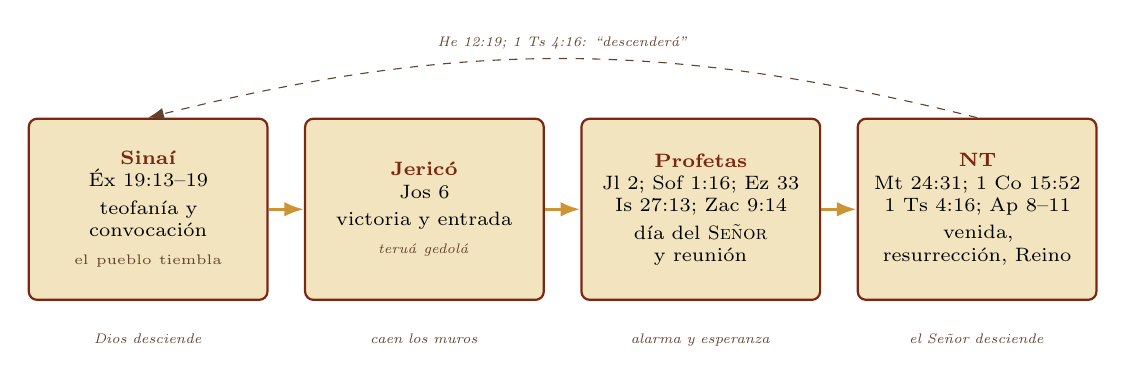
\begin{tikzpicture}[font=\scriptsize,node distance=0.45cm]
 \tikzset{et/.style={draw=tierraroja,line width=0.8pt,fill=papiro,rounded corners=3pt,text width=2.75cm,align=center,inner sep=4pt,minimum height=2.3cm}}
 \node[et] (s) {\textbf{\textcolor{tierraroja}{Sinaí}}\\ Éx 19:13--19\\[2pt] teofanía y convocación\\[2pt] {\tiny\color{sepia}el pueblo tiembla}};
 \node[et,right=of s] (j) {\textbf{\textcolor{tierraroja}{Jericó}}\\ Jos 6\\[2pt] victoria y entrada\\[2pt] {\tiny\color{sepia}\emph{teruá gedolá}}};
 \node[et,right=of j] (p) {\textbf{\textcolor{tierraroja}{Profetas}}\\ Jl 2; Sof 1:16; Ez 33\\ Is 27:13; Zac 9:14\\[2pt] día del \SENOR{} y reunión};
 \node[et,right=of p] (n) {\textbf{\textcolor{tierraroja}{NT}}\\ Mt 24:31; 1 Co 15:52\\ 1 Ts 4:16; Ap 8--11\\[2pt] venida, resurrección, Reino};
 \foreach \a/\b in {s/j,j/p,p/n}{\draw[-{Latex[length=2.5mm]},mostaza!90!tierraroja,line width=1.2pt] (\a)--(\b);}
 \node[below=0.3cm of s,text width=2.75cm,align=center,font=\tiny\itshape,text=sepia] {Dios desciende};
 \node[below=0.3cm of j,text width=2.75cm,align=center,font=\tiny\itshape,text=sepia] {caen los muros};
 \node[below=0.3cm of p,text width=2.75cm,align=center,font=\tiny\itshape,text=sepia] {alarma y esperanza};
 \node[below=0.3cm of n,text width=2.75cm,align=center,font=\tiny\itshape,text=sepia] {el Señor desciende};
 \draw[sepia,dashed,-{Latex[length=2mm]}] (n.north) to[bend right=14] node[midway,above,font=\tiny\itshape,text=sepia]{He 12:19; 1 Ts 4:16: ``descenderá''} (s.north);
\end{tikzpicture}\par
{\footnotesize\color{sepia}\textit{Figura 9.} Trayectoria de la trompeta en el canon. \textit{Nota.} Elaboración propia. La flecha discontinua marca el retorno del motivo del descenso: en el Sinaí Dios desciende al son del \emph{shofar} (Éx 19:18, 20); en 1~Ts 4:16 el Señor ``descenderá del cielo'' con trompeta de Dios.}
\end{minipage}\end{center}

La trayectoria muestra que el Nuevo Testamento no inventa la trompeta escatológica: la hereda de los profetas, que ya habían leído el \emph{shofar} del Sinaí y de la guerra santa como la señal del día en que Dios interviene. El vínculo con la fiesta del mes séptimo es léxico (\emph{yom teruá}, \emph{yom shofar uteruá}) y temático, no siempre explícito.

%===================================================================
\section{Memorial, figura y esperanza: la lectura de la serie}

\subsection{La pregunta del documento: ¿por qué ``conmemoración''?}
El documento de referencia de la serie (lecciones 8 y 12) parte de un detalle que ``no siempre se le da importancia'': Lv 23:24 llama a la fiesta ``conmemoración''. Cuando la ley se daba en el Sinaí, observa, Israel ``aún estaba lejos de imaginar siquiera lo que sería la vida futura de la nación''. ¿Qué hecho podía conmemorar una fiesta instituida antes de que ocurriera? La respuesta del documento: la generación del desierto la conocería ``cuarenta y un años más tarde'', al rodear la ciudad que era ``la puerta de entrada a la Tierra Prometida''. La Fiesta de las Trompetas representa para Israel ``el momento maravilloso cuando Dios con su poder, y \emph{al son de Trompetas}, derribó los muros de Jericó''.

El documento atribuye a ese toque tres significados: primero, que había llegado el momento de la heredad prometida a Abraham, Isaac y Jacob; segundo, que ``sus faltas habían sido purgadas'', que había concluido el juicio divino contra la generación rebelde del desierto; tercero, que había llegado el momento de entrar en la tierra. Esos tres hechos corresponden a las tres convocaciones del mes séptimo, y el documento los dispone en una tabla que la Tabla~3 reproduce y completa con la lectura del Nuevo Pacto.

\begin{center}\begin{minipage}{\linewidth}\centering\small\renewcommand{\arraystretch}{1.18}
\begin{tabular}{@{}L{4.2cm}L{3.4cm}L{6.8cm}@{}}
\toprule
\textbf{La historia de Israel} & \textbf{El Reglamento de Culto} & \textbf{El Nuevo Pacto (lectura de la serie)} \\ \midrule
Israel salvado de la muerte & Pascua & Cristo nuestra Pascua (1~Co 5:7) \\
Israel libre del cautiverio & Ázimos & la Iglesia sin levadura (1~Co 5:8) \\
La entrega de la Ley & Pentecostés & el derramamiento del Espíritu (Hch 2) \\
\textbf{La toma de Jericó} & \textbf{Trompetas} & \textbf{el regreso de Cristo a la final trompeta (1~Co 15:51--53; 1~Ts 4:15--17; Ap 10:7; 11:15)} \\
Fin del juicio en el desierto & Expiación & fin del juicio a la casa de Dios (1~P 4:17); Satanás atado (Ap 20:1--3) \\
Israel entra en Canaán & Cabañas & el Reino milenial (Ap 20:4--6) \\
\bottomrule
\end{tabular}\par
{\footnotesize\color{sepia}\textit{Tabla 3.} Historia de Israel, Reglamento de Culto y Nuevo Pacto. \textit{Nota.} Las dos primeras columnas reproducen la tabla de la lección 12 del documento de referencia; la tercera resume las lecciones 8, 12--14.}
\end{minipage}\end{center}

\subsection{La figura: Jericó y la Iglesia}
La presentación de Danilo enmarca la fiesta en el Dios de pactos: los gentiles estaban ``ajenos a los pactos de la promesa'' (\grc{τῶν διαθηκῶν τῆς ἐπαγγελίας}, Ef 2:12) y en Cristo han sido acercados; las convocaciones del pacto con Israel se vuelven así herencia de la Iglesia. 
El nexo con la Iglesia, dice el documento, ``subyace necesariamente en la historia del Pueblo de Israel'', porque la existencia de la nación y su desarrollo ``prefiguran la presencia y desarrollo de este Israel espiritual''. Para la Iglesia también hay un Reino prometido (Jn 14:1--3), y llegará ``del mismo modo'' que para Israel: precedido del sonido de trompetas (1~Ts 4:15--17) y no antes de que concluya ``el juicio ya presente entre sus miembros'' (1~P 4:17). El documento reúne tres textos:

\begin{cita}He aquí, os digo un misterio: No todos dormiremos; pero todos seremos transformados, en un momento, en un abrir y cerrar de ojos, a la final trompeta; porque se tocará la trompeta, y los muertos serán resucitados incorruptibles, y nosotros seremos transformados.\fuente{(1~Co 15:51--52)}\end{cita}

\begin{cita}Porque el Señor mismo con voz de mando, con voz de arcángel, y con trompeta de Dios, descenderá del cielo; y los muertos en Cristo resucitarán primero. Luego nosotros los que vivimos, los que hayamos quedado, seremos arrebatados juntamente con ellos en las nubes para recibir al Señor en el aire, y así estaremos siempre con el Señor.\fuente{(1~Ts 4:16--17)}\end{cita}

\begin{cita}\ldots{}sino que en los días de la voz del séptimo ángel, cuando él comience a tocar la trompeta, el misterio de Dios se consumará, como él lo anunció a sus siervos los profetas.\fuente{(Ap 10:7)}\end{cita}

``Entre otras muchas Escrituras'', concluye, ``estas tres enfocan un acontecimiento majestuoso al son de trompeta que no es otra cosa que el regreso de Nuestro Señor Jesús para establecer su Reino y congregar su pueblo''. La fiesta lo simboliza, y por eso su observancia ``testimonia nuestra esperanza''. La séptima trompeta de Apocalipsis completa el cuadro: ``Los reinos del mundo han venido a ser de nuestro Señor y de su Cristo; y él reinará por los siglos de los siglos'' (Ap 11:15). La Figura~10 muestra la correspondencia de las tres fiestas del otoño en esta lectura.

\begin{center}\begin{minipage}{\linewidth}\centering
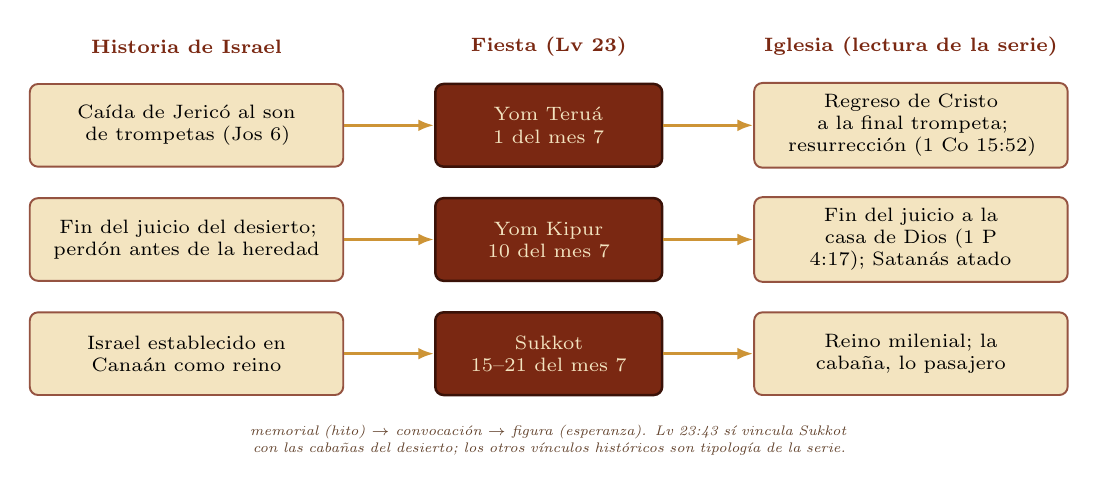
\begin{tikzpicture}[font=\scriptsize]
 \tikzset{c/.style={draw=tierraroja!80,line width=0.7pt,fill=papiro,rounded corners=3pt,text width=3.7cm,align=center,inner sep=4pt,minimum height=1.05cm}}
 \tikzset{f/.style={draw=caferojizo,line width=0.9pt,fill=tierraroja,text=papiro,rounded corners=3pt,text width=2.6cm,align=center,inner sep=4pt,minimum height=1.05cm}}
 \node[font=\scriptsize\bfseries,text=tierraroja] at (0,1.0) {Historia de Israel};
 \node[font=\scriptsize\bfseries,text=tierraroja] at (4.6,1.0) {Fiesta (Lv 23)};
 \node[font=\scriptsize\bfseries,text=tierraroja] at (9.2,1.0) {Iglesia (lectura de la serie)};
 \foreach \k/\y/\h/\fe/\ig in {1/0/{Caída de Jericó al son de trompetas (Jos 6)}/{Yom Teruá\\ 1 del mes 7}/{Regreso de Cristo a la final trompeta; resurrección (1 Co 15:52)},
  2/-1.45/{Fin del juicio del desierto; perdón antes de la heredad}/{Yom Kipur\\ 10 del mes 7}/{Fin del juicio a la casa de Dios (1 P 4:17); Satanás atado},
  3/-2.9/{Israel establecido en Canaán como reino}/{Sukkot\\ 15--21 del mes 7}/{Reino milenial; la cabaña, lo pasajero}}{
   \node[c] (h\k) at (0,\y) {\h};
   \node[f] (f\k) at (4.6,\y) {\fe};
   \node[c] (i\k) at (9.2,\y) {\ig};
   \draw[-{Latex[length=2mm]},mostaza!90!tierraroja,line width=1pt] (h\k)--(f\k);
   \draw[-{Latex[length=2mm]},mostaza!90!tierraroja,line width=1pt] (f\k)--(i\k);}
 \node[text width=13cm,align=center,font=\tiny\itshape,text=sepia] at (4.6,-4.0) {memorial (hito) $\rightarrow$ convocación $\rightarrow$ figura (esperanza). Lv 23:43 sí vincula Sukkot con las cabañas del desierto; los otros vínculos históricos son tipología de la serie.};
\end{tikzpicture}\par
{\footnotesize\color{sepia}\textit{Figura 10.} Las tres convocaciones del mes séptimo en la lectura de la serie. \textit{Nota.} Elaboración propia a partir de las lecciones 8 y 12--14 del documento de referencia.}
\end{minipage}\end{center}

\subsection{Lo que la Escritura sostiene de esta lectura}
La lectura de la serie tiene apoyo bíblico en varios puntos, y conviene nombrarlos:

\begin{enumerate}\setlength{\itemsep}{2pt}
\item \textbf{El vocabulario es el mismo.} La \emph{teruá gedolá} de Jericó (Jos 6:5, 20) es la \emph{teruá} de Lv 23:24 y Nm 29:1. Un lector hebreo oye la fiesta en el relato y el relato en la fiesta.
\item \textbf{El Nuevo Testamento lee tipológicamente a Josué.} Hebreos compara el reposo que ``Josué'' no dio con el reposo que queda para el pueblo de Dios (He 4:8--9), y en griego ``Josué'' es \grc{Ἰησοῦς}, el mismo nombre de Jesús. La forma \heb{יֵשׁוּעַ} (\emph{Yeshúa}) se aplica al propio Josué hijo de Nun en Neh 8:17, precisamente en el relato de la fiesta del mes séptimo.
\item \textbf{La trompeta de la venida es la trompeta de la guerra santa.} 1~Ts 4:16 y Ap 8--11 usan la trompeta como señal de la intervención de Dios contra sus enemigos y a favor de su pueblo, como en Nm 10:9 (``seréis salvos de vuestros enemigos'') y en Jericó. Algunos comentaristas reconocen el fondo de Jos 6 en las siete trompetas del Apocalipsis (Beale, 1999).
\item \textbf{La secuencia del otoño es escatológica en los profetas.} Zacarías 14, que el documento cita para el descenso en el monte de los Olivos (Zac 14:4--5), termina con las naciones subiendo a Jerusalén ``para celebrar la fiesta de los tabernáculos'' (14:16). Los profetas ya leían el final del calendario como el final de la historia.
\end{enumerate}

\clearpage
\subsection{Precisiones}
El respeto por la lectura de la serie exige marcar también lo que el texto no dice.

\begin{nota}[Precisión: el hito conmemorado]
\textbf{1.} Lv 23 no dice qué hecho conmemora la fiesta, y ningún texto bíblico la relaciona con Jericó. La conexión es tipología de la serie. \textbf{2.} Según Jos 4:19 y 5:10, Jericó cayó en el mes primero, días después de Pésaj, no el primer día del mes séptimo (véase §3.4). \textbf{3.} La propia Escritura ofrece otra explicación de \emph{zijrón teruá}: en Nm 10:9--10 la memoria va hacia Dios (``seréis recordados por \SENOR''). Las dos lecturas no se excluyen: el toque presenta a Israel ante Dios, y Jericó es el gran ejemplo narrativo de lo que Nm 10:9 promete (``seréis salvos de vuestros enemigos''). \textbf{4.} Filón ya buscó un hito histórico para la fiesta, pero propuso otro: el Sinaí (\emph{Spec.} 2.188--189). Que la tradición proponga hitos distintos confirma que el texto no lo fija.
\end{nota}

\begin{nota}[Precisión: la secuencia y las citas]
\textbf{1.} En el libro de Josué el orden es otro: el cruce del Jordán y la entrada en la tierra (Jos 3--4) preceden a Jericó (Jos 6), y el pecado de Acán (Jos 7) muestra que el juicio no había ``concluido'' con la caída de la ciudad. La correspondencia Expiación--fin del juicio y Cabañas--entrada en Canaán es tipológica; Lv 23:43 vincula Sukkot con las cabañas del desierto, no con la entrada. \textbf{2.} La cita de 1~Ts 4:16 del documento (``con aclamación'') sigue una versión anterior, como la Reina-Valera de 1909; la RVR1960 dice ``con voz de mando'' (\grc{ἐν κελεύσματι}). \textbf{3.} En Jericó suenan \emph{shofarot}, no las \emph{jatsotsrot} de plata de Nm 10. \textbf{4.} La identificación de la fiesta con ``la salida de nuestro Sumo Pontífice del Lugar Santísimo'' (lección 13) pertenece al estudio de Yom Kipur y se trata allí.
\end{nota}

%===================================================================
\section{La fiesta en Jesús y los apóstoles}

\subsection{Los evangelios}
Los evangelios no mencionan Yom Teruá por su nombre. Juan 5:1 habla de ``una fiesta de los judíos'' sin identificarla, y algunos intérpretes han propuesto esta (es una minoría: otros piensan en Pésaj, Purim o Sukkot). Lo que sí aparece es la trompeta escatológica en el discurso del monte de los Olivos:

\begin{cita}Y enviará sus ángeles con gran voz de trompeta, y juntarán a sus escogidos, de los cuatro vientos, desde un extremo del cielo hasta el otro.\fuente{(Mt 24:31)}\end{cita}

La ``gran trompeta'' (\grc{σάλπιγγος μεγάλης}) es el \emph{shofar gadol} de Is 27:13 (LXX \grc{τῇ σάλπιγγι τῇ μεγάλῃ}), el que reúne a los dispersos; ``los cuatro vientos'' evoca Zac 2:6 [2:10], y ``desde un extremo del cielo'' recuerda Dt 30:4. Jesús toma la imagen profética de la reunión de Israel y la aplica a la reunión de ``sus escogidos'' por el Hijo del Hombre. La décima bendición de la oración judía de las Dieciocho Bendiciones usa la misma imagen: ``Toca el gran \emph{shofar} para nuestra libertad, y alza bandera para reunir a nuestros desterrados'' (trad. propia; texto litúrgico de fecha discutida). El discurso no menciona ninguna fiesta; el eco es profético. Sobre Mt 24:36, véase la precisión de §5.4.

\subsection{Pablo: 1 Corintios 15}
En 1~Co 15 Pablo cierra su argumento sobre la resurrección con un ``misterio'': no todos morirán, pero todos serán transformados, ``en un momento (\grc{ἐν ἀτόμῳ}), en un abrir y cerrar de ojos, a la final trompeta (\grc{ἐν τῇ ἐσχάτῃ σάλπιγγι})'' (15:51--52). La palabra ``final'' (\grc{ἐσχάτη}) es escatológica: designa la trompeta del fin, no necesariamente la última de una serie contada (Fee, 1987). Pablo une el sonido con la victoria sobre la muerte, y lo sella con dos citas proféticas: ``Sorbida es la muerte en victoria'' (Is 25:8) y ``¿Dónde está, oh muerte, tu aguijón?'' (Os 13:14). La trompeta de la guerra santa (Nm 10:9) anuncia aquí la derrota del último enemigo (1~Co 15:26).

\subsection{Pablo: 1 Tesalonicenses 4:13--18}
Los tesalonicenses temían que sus muertos quedaran excluidos de la venida del Señor. Pablo responde con una ``palabra del Señor'' (4:15) que tiene una estructura nítida (Figura~11): tres sonidos acompañan el descenso, y el descenso produce dos movimientos, la resurrección de los muertos y el arrebatamiento de los vivos, que terminan en un encuentro y una permanencia.

\begin{center}\begin{minipage}{\linewidth}\centering
\begin{tikzpicture}[font=\scriptsize]
 \tikzset{v/.style={draw=tierraroja!80,line width=0.7pt,fill=papiro,rounded corners=3pt,text width=3.3cm,align=center,inner sep=4pt,minimum height=1.0cm}}
 \node[v] (v1) at (0,0) {\grc{ἐν κελεύσματι}\\ ``con voz de mando''};
 \node[v] (v2) at (4.5,0) {\grc{ἐν φωνῇ ἀρχαγγέλου}\\ ``con voz de arcángel''};
 \node[v] (v3) at (9,0) {\grc{ἐν σάλπιγγι θεοῦ}\\ ``con trompeta de Dios''};
 \node[draw=caferojizo,fill=tierraroja,text=papiro,rounded corners=3pt,text width=6.8cm,align=center,inner sep=5pt] (d) at (4.5,-1.55) {\textbf{\grc{αὐτὸς ὁ κύριος} \ldots{} \grc{καταβήσεται ἀπ᾽ οὐρανοῦ}}\\ ``el Señor mismo descenderá del cielo'' (4:16)};
 \foreach \n in {v1,v2,v3}{\draw[-{Latex[length=2mm]},mostaza!90!tierraroja,line width=1pt] (\n.south) -- (d.north);}
 \node[v] (r1) at (1.6,-3.2) {los muertos en Cristo resucitarán \textbf{primero} (4:16)};
 \node[v] (r2) at (7.4,-3.2) {los vivos serán \textbf{arrebatados} juntamente con ellos (4:17)};
 \draw[-{Latex[length=2mm]},mostaza!90!tierraroja,line width=1pt] (d) -- (r1);
 \draw[-{Latex[length=2mm]},mostaza!90!tierraroja,line width=1pt] (d) -- (r2);
 \node[draw=tierraroja,line width=1pt,fill=mostaza!25,rounded corners=3pt,text width=6.8cm,align=center,inner sep=5pt] (e) at (4.5,-4.75) {\grc{εἰς ἀπάντησιν τοῦ κυρίου εἰς ἀέρα}: ``para recibir al Señor en el aire''\\ \grc{καὶ οὕτως πάντοτε σὺν κυρίῳ ἐσόμεθα} (4:17)};
 \draw[-{Latex[length=2mm]},mostaza!90!tierraroja,line width=1pt] (r1) -- (e);
 \draw[-{Latex[length=2mm]},mostaza!90!tierraroja,line width=1pt] (r2) -- (e);
\end{tikzpicture}\par
{\footnotesize\color{sepia}\textit{Figura 11.} Estructura de 1~Ts 4:16--17. \textit{Nota.} Elaboración propia con NA28 y la RVR1960.}
\end{minipage}\end{center}

Tres detalles del griego importan. \grc{Κέλευσμα} es la voz de mando militar. \grc{Σάλπιγξ θεοῦ}, ``trompeta de Dios'', puede leerse como ``la trompeta que pertenece a Dios'' o ``la que Dios toca'', como en Zac 9:14. Y \grc{ἀπάντησις} designaba en el mundo helenístico la salida de los ciudadanos al encuentro de un dignatario que llega, para escoltarlo de vuelta a la ciudad; muchos intérpretes leen así el ``encuentro en el aire'': la Iglesia sale a recibir al Rey que viene a la tierra (Wright, 2003; Fee, 2009). Esta lectura es coherente con la de la serie (el Señor que viene a establecer su Reino) y discute la del arrebatamiento a un lugar celestial fuera de la tierra.

\subsection{Hebreos: del Sinaí a Sion}
Hebreos contrasta dos montes. Los creyentes no se han acercado al monte que se podía palpar, ``al sonido de la trompeta, y a la voz que hablaba'' (He 12:19), sino ``al monte de Sion, a la ciudad del Dios vivo, Jerusalén la celestial'' (12:22). La trompeta del Sinaí queda como advertencia: el que habló entonces ``conmovió la tierra'', y ha prometido conmover ``no solamente la tierra, sino también el cielo'' (12:26, citando Hag 2:6).

\begin{nota}[Precisión: Hebreos]
El documento de referencia atribuye Hebreos al apóstol Pablo, y así se respeta su voz al exponerlo. La autoría de la carta es discutida desde la Iglesia antigua; la mayoría de los comentarios actuales la consideran anónima (Attridge, 1989; Lane, 1991). El argumento de este capítulo no depende de la autoría.
\end{nota}

\subsection{Apocalipsis: la voz como de trompeta y las siete trompetas}
Juan oye ``en el día del Señor'' una ``gran voz como de trompeta'' (Ap 1:10), y la misma voz lo llama a subir: ``Sube acá, y yo te mostraré las cosas que sucederán'' (4:1). Como en el Sinaí, la trompeta es la voz que convoca a la presencia de Dios. En los capítulos 8--11, siete ángeles reciben siete trompetas (8:2). Las cuatro primeras hieren un tercio de la tierra, del mar, de las aguas y de los astros (8:7--12), con ecos de las plagas de Egipto (granizo y fuego, agua en sangre, tinieblas). Un águila anuncia tres ayes (8:13): la quinta trompeta trae las langostas del abismo (9:1--11) y la sexta, los ejércitos del Éufrates (9:13--21). Entre la sexta y la séptima hay un interludio: el ángel del librito, que jura que ``el misterio de Dios se consumará'' cuando suene la séptima (10:7), y los dos testigos (11:1--14). La séptima trompeta proclama el reino: \grc{ἐγένετο ἡ βασιλεία τοῦ κόσμου τοῦ κυρίου ἡμῶν καὶ τοῦ Χριστοῦ αὐτοῦ}, ``el reino del mundo ha venido a ser de nuestro Señor y de su Cristo'' (11:15; el griego dice ``reino'' en singular), y se abre el templo de Dios en el cielo, y ``el arca de su pacto se veía en el templo'' (11:19).

\begin{center}\begin{minipage}{\linewidth}\centering
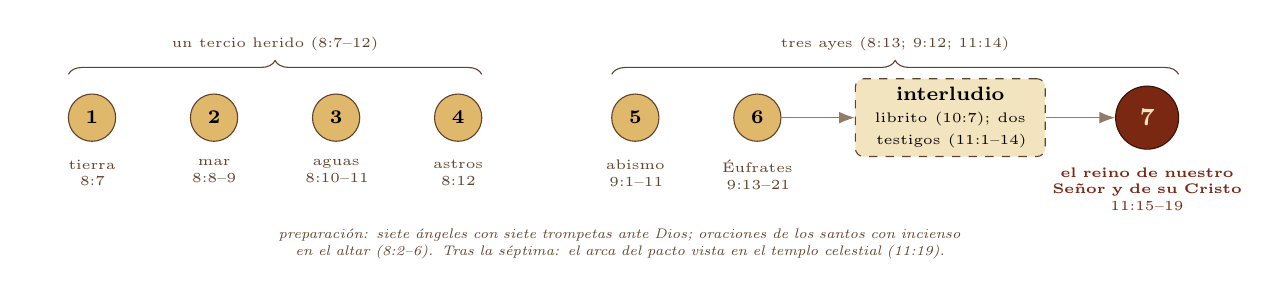
\begin{tikzpicture}[font=\scriptsize]
 \foreach \n/\x/\t in {1/0/{tierra\\ 8:7},2/1.55/{mar\\ 8:8--9},3/3.1/{aguas\\ 8:10--11},4/4.65/{astros\\ 8:12},5/6.9/{abismo\\ 9:1--11},6/8.45/{Éufrates\\ 9:13--21}}{
   \node[circle,fill=mostaza!75,draw=sepia,minimum size=6mm,font=\scriptsize\bfseries] (t\n) at (\x,0) {\n};
   \node[below=3pt,text width=1.4cm,align=center,font=\tiny,text=sepia] at (t\n.south) {\t};}
 \node[draw=sepia,dashed,rounded corners=3pt,fill=papiro,text width=2.2cm,align=center,inner sep=3pt] (int) at (10.9,0) {\textbf{interludio}\\ {\tiny librito (10:7); dos testigos (11:1--14)}};
 \node[circle,fill=tierraroja,draw=caferojizo,minimum size=8mm,text=papiro,font=\small\bfseries] (t7) at (13.4,0) {7};
 \node[below=3pt,text width=2.4cm,align=center,font=\tiny,text=tierraroja] at (t7.south) {\textbf{el reino de nuestro Señor y de su Cristo}\\ 11:15--19};
 \draw[decorate,decoration={brace,amplitude=5pt},sepia] (-0.3,0.55) -- (4.95,0.55) node[midway,above=5pt,font=\tiny,text=sepia] {un tercio herido (8:7--12)};
 \draw[decorate,decoration={brace,amplitude=5pt},sepia] (6.6,0.55) -- (13.8,0.55) node[midway,above=5pt,font=\tiny,text=sepia] {tres ayes (8:13; 9:12; 11:14)};
 \draw[-{Latex[length=2mm]},sepia!70] (t6) -- (int); \draw[-{Latex[length=2mm]},sepia!70] (int) -- (t7);
 \node[text width=14cm,align=center,font=\tiny\itshape,text=sepia] at (6.7,-1.6) {preparación: siete ángeles con siete trompetas ante Dios; oraciones de los santos con incienso en el altar (8:2--6). Tras la séptima: el arca del pacto vista en el templo celestial (11:19).};
\end{tikzpicture}\par
{\footnotesize\color{sepia}\textit{Figura 12.} Las siete trompetas de Apocalipsis 8--11. \textit{Nota.} Elaboración propia con NA28.}
\end{minipage}\end{center}

Bauckham (1993) mostró que las series de siete del Apocalipsis (sellos, trompetas, copas) están entrelazadas y que los juicios de las trompetas son parciales (``la tercera parte'') y no logran el arrepentimiento: los sobrevivientes ``ni aun así se arrepintieron'' (9:20--21). Lo que sí produce conversión es el testimonio de los dos testigos: tras su vindicación, ``los demás se aterrorizaron, y dieron gloria al Dios del cielo'' (11:13). La séptima trompeta no es otro juicio, sino el anuncio del reino. Para esta fiesta, el dato es significativo: la trompeta del fin, como la del Sinaí y la de Jericó, convoca, juzga y proclama el reinado de Dios. Que la séptima trompeta muestre ``el arca de su pacto'' (11:19) enlaza además con la fiesta siguiente, Yom Kipur, el único día en que el sumo sacerdote veía el arca.

\subsection{¿Cuál es la final trompeta?}
La presentación de Danilo sobre Yom Teruá plantea la pregunta directamente: si Pablo habla de ``la final trompeta'' (1~Co 15:52), ¿cuál es? Su respuesta recorre el Apocalipsis: los siete sellos (Ap 6--8:1), cuyo séptimo sello abre, tras ``silencio en el cielo como por media hora'', las siete trompetas (8:1--2), y la séptima de ellas, que proclama el reino (11:15). La Tabla~4 sigue ese recorrido.

\begin{center}\begin{minipage}{\linewidth}\centering\small\renewcommand{\arraystretch}{1.14}
\begin{tabular}{@{}L{1.0cm}L{6.3cm}L{1.0cm}L{6.1cm}@{}}
\toprule
\multicolumn{2}{@{}l}{\textbf{Siete sellos (Ap 6:1--8:1)}} & \multicolumn{2}{l@{}}{\textbf{Siete trompetas (Ap 8:2--11:19)}} \\ \midrule
1 & caballo blanco: el que vence (6:2) & 1 & granizo y fuego; un tercio de la tierra (8:7) \\
2 & caballo bermejo: la guerra (6:4) & 2 & monte ardiendo en el mar (8:8--9) \\
3 & caballo negro: la balanza, la carestía (6:5--6) & 3 & la estrella Ajenjo, aguas amargas (8:10--11) \\
4 & caballo amarillo: la muerte (6:8) & 4 & un tercio del sol, la luna y las estrellas (8:12) \\
5 & las almas bajo el altar (6:9--11) & 5 & primer ay: langostas del abismo; Abadón/Apolión (9:1--12) \\
6 & sol oscurecido, luna como sangre (6:12--17; cf. Is 13:9--11; Jl 2:1--2; Mt 24:29) & 6 & segundo ay: los ángeles del Éufrates; doscientos millones (9:13--21) \\
7 & silencio; siete ángeles con trompetas; el incensario (8:1--5) & 7 & ``los reinos del mundo'' son del Señor; juicio de los muertos, galardón; el arca del pacto (11:15--19) \\
\bottomrule
\end{tabular}\par
{\footnotesize\color{sepia}\textit{Tabla 4.} De los sellos a la séptima trompeta. \textit{Nota.} Elaboración propia a partir de la presentación de Danilo (``Yom Teruá'') y NA28.}
\end{minipage}\end{center}

La séptima trompeta reúne lo que Pablo asocia con la trompeta final: el tiempo de ``juzgar a los muertos'' y de ``dar el galardón a tus siervos los profetas, a los santos'' (Ap 11:18), y el reino del Señor y de su Cristo (11:15; cf. 1~Co 15:24--26, 52). Danilo la lee junto con Mt 24:30--31 (el Hijo del Hombre sobre las nubes, la gran trompeta) y con Daniel: el Hijo del Hombre que recibe ``dominio, gloria y reino'' (Dn 7:13--14) y el tiempo en que ``muchos de los que duermen en el polvo de la tierra serán despertados'' (Dn 12:2). La lectura de la serie coincide: los que resuciten o sean transformados ``al sonido de la séptima trompeta (1~Co 15:51--53)'' son la Iglesia en el regreso del Señor (documento de referencia, lección 13).

\begin{nota}[Precisión: ``final'' y ``séptima'']
Identificar la ``final trompeta'' de 1~Co 15:52 con la séptima de Ap 11:15 es una lectura canónica coherente, sostenida por la serie y por muchos intérpretes, pero no explícita: 1~Corintios es anterior al Apocalipsis y no cuenta trompetas. Otros entienden \grc{ἐσχάτη} como ``escatológica'', la trompeta del fin, sin referencia a una serie (Fee, 1987). Las dos lecturas coinciden en lo esencial: la trompeta final acompaña la resurrección y el reino.
\end{nota}

\subsection{El día del despertar}
En otra de sus presentaciones (``La fiesta del séptimo mes''), Danilo desarrolla una imagen que la tradición judía también conoce: Yom Teruá como \destacar{día del despertar}. El \emph{shofar} es una alarma que despierta y convoca: llama a congregarse (Nm 10:2--3), llama al arrepentimiento (``alza tu voz como trompeta, y anuncia a mi pueblo su rebelión'', Is 58:1) y llama a la resurrección. Los textos que reúne forman una cadena profética:

\begin{cita}Tus muertos vivirán; sus cadáveres resucitarán. ¡Despertad y cantad, moradores del polvo! porque tu rocío es cual rocío de hortalizas, y la tierra dará sus muertos.\fuente{(Is 26:19)}\end{cita}

Isaías 25:8 anuncia que Dios ``destruirá a la muerte para siempre'', el versículo que Pablo cita junto a la trompeta final (1~Co 15:54). Isaías 42:10--13 convoca a cantar ``un nuevo cántico'' y describe al \SENOR{} que ``gritará, voceará'' (\heb{יָרִיעַ}, de la raíz de \emph{teruá}) contra sus enemigos: el grito del guerrero divino. Isaías 12 es el canto del día de la salvación. Oseas 9:5 pregunta: ``¿Qué haréis en el día de la solemnidad, y en el día de la fiesta de \SENOR?''. Y el Salmo 89:15--16 [89:16--17] da la respuesta positiva: bienaventurado el pueblo ``que sabe aclamarte''; ``en tu nombre se alegrará todo el día''.

Danilo lee además dos textos de Efesios en esta clave. ``Despiértate, tú que duermes, y levántate de los muertos, y te alumbrará Cristo'' (Ef 5:14) suena como un toque de despertar, y ``fuisteis sellados para el día de la redención'' (Ef 4:30) apunta al día de la venida. La lectura es sugerente y debe marcarse como posible eco.

\begin{nota}[Precisión: Efesios y el despertar]
Ef 5:14 se introduce con ``por lo cual dice'' y parece citar un himno cristiano primitivo que combina Is 26:19 y 60:1; no menciona trompetas ni fiestas. El vínculo con Yom Teruá es un eco posible por la vía de Is 26:19 (despertar de los muertos) y de Maimónides (``despertad, dormidos''), no una alusión demostrable. La autoría paulina de Efesios es discutida; el argumento se apoya también en cartas indiscutidas (1~Co 15:52; 1~Ts 4:16).
\end{nota}

%===================================================================
\section{La fiesta en la tradición judía}

\begin{nota}[Precisión]
Esta sección describe la tradición rabínica (Misná, Talmud, liturgia del \emph{sidur} y del \emph{majzor}) y prácticas posteriores. Son testimonio de cómo el judaísmo leyó la fiesta, no contenido explícito de la Torá.
\end{nota}

\subsection{De Yom Teruá a Rosh haShaná}
La Misná dedica un tratado entero a la fiesta, \emph{Rosh haShaná}, y fija tres ideas. La primera es el año nuevo (1:1, véase §5.2). La segunda es el juicio: ``En cuatro tiempos el mundo es juzgado: en Pésaj, por el grano; en Atséret, por los frutos del árbol; en Rosh haShaná todos los que vienen al mundo pasan delante de Él como \emph{bené marón}'', una expresión de sentido discutido (ovejas en fila, soldados, o los que suben una cuesta estrecha) (1:2). La tercera es el \emph{shofar} como precepto central del día (3:3--4:9). El Talmud añade la imagen de los tres libros abiertos en Rosh haShaná: los justos son inscritos para la vida, los malvados para la muerte, y los intermedios quedan en suspenso hasta Yom Kipur (b.~\emph{Rosh haShaná} 16b). De ahí nacen los \emph{yamim noraim}, los ``días temibles'', o \emph{aséret yemé teshuvá}, los diez días de arrepentimiento que van del 1 al 10 de Tishri.

\subsection{La liturgia del shofar}
La oración adicional (\emph{musaf}) del día tiene tres bendiciones centrales, cada una con diez versículos bíblicos (\emph{Rosh haShaná} 4:5--6):

\begin{center}\begin{minipage}{\linewidth}\centering\small\renewcommand{\arraystretch}{1.18}
\begin{tabular}{@{}L{2.6cm}L{5.0cm}L{6.8cm}@{}}
\toprule
\textbf{Bendición} & \textbf{Tema} & \textbf{Fundamento bíblico (ejemplos)} \\ \midrule
\heb{מַלְכֻיּוֹת} \emph{maljuyot} & la realeza de Dios & Nm 23:21 (``júbilo de rey en él''); Sal 24; Sal 47; Sal 98:6 \\
\heb{זִכְרוֹנוֹת} \emph{zijronot} & Dios que recuerda & Gn 8:1 (Noé); Éx 2:24 (el pacto); Lv 26:42; Jer 2:2; Jer 31:20 \\
\heb{שׁוֹפָרוֹת} \emph{shofarot} & el \emph{shofar} de la historia & Éx 19:16, 19 (Sinaí); Sal 81:3; Is 27:13; Zac 9:14 \\
\bottomrule
\end{tabular}\par
{\footnotesize\color{sepia}\textit{Tabla 5.} Las tres bendiciones del \emph{musaf} de Rosh haShaná. \textit{Nota.} Elaboración propia con la Misná (\emph{Rosh haShaná} 4:5--6) y el \emph{majzor}; la selección de versículos es posterior a la Misná.}
\end{minipage}\end{center}

El Talmud resume el sentido de las tres en una frase atribuida a Dios: ``Decid delante de mí \emph{maljuyot}, para que me hagáis rey sobre vosotros; \emph{zijronot}, para que vuestro recuerdo suba ante mí para bien; ¿y con qué? Con el \emph{shofar}'' (b.~\emph{Rosh haShaná} 16a, trad. propia). Las tres bendiciones recogen los tres sentidos que la filología encontró en \emph{teruá}: aclamación del rey, memoria ante Dios y señal de su intervención.

Los toques también se codificaron. La Misná exige tres series de tres toques: \emph{tekiá} (toque largo), \emph{teruá}, \emph{tekiá} (\emph{Rosh haShaná} 4:9). Como no se sabía con exactitud qué sonido era la \emph{teruá} bíblica, si un gemido o un sollozo, el Talmud atribuye a Rabí Abahu, en Cesarea, la combinación que aún se usa: \emph{tekiá}, \emph{shevarim} (tres toques quebrados, el ``gemido'') y \emph{teruá} (nueve toques breves, el ``sollozo'') (b.~\emph{Rosh haShaná} 34a). El último toque del día se prolonga: la \emph{tekiá guedolá}.

\subsection{Las lecturas y la \emph{aqedá}}
El primer día se lee Génesis 21 (``Visitó \SENOR{} a Sara'') y, como \emph{haftará}, 1~Samuel 1:1--2:10 (``\SENOR{} se acordó de ella'', 1:19): dos madres estériles recordadas por Dios. El segundo día se lee Génesis 22, la \emph{aqedá} o atadura de Isaac, y Jeremías 31:2--20, que culmina en ``me acuerdo de él constantemente'' (\heb{זָכֹר אֶזְכְּרֶנּוּ עוֹד}, Jer 31:20). El cuerno de carnero se explica por el carnero ``trabado en un zarzal por sus cuernos'' (Gn 22:13): ``Tocad delante de mí con cuerno de carnero, para que recuerde a vuestro favor la atadura de Isaac'' (b.~\emph{Rosh haShaná} 16a, trad. propia). La lectura judía y la cristiana se cruzan aquí: la Iglesia ha leído la \emph{aqedá} como figura del Padre que no escatimó a su Hijo (Ro 8:32).

\subsection{Las notas del shofar}
La presentación de Danilo asocia cada toque del \emph{shofar} con un texto bíblico. La Tabla~6 la recoge.

\begin{center}\begin{minipage}{\linewidth}\centering\small\renewcommand{\arraystretch}{1.16}
\begin{tabular}{@{}L{3.4cm}L{5.2cm}L{5.8cm}@{}}
\toprule
\textbf{Toque} & \textbf{Descripción (tradición)} & \textbf{Texto asociado (presentación de Danilo)} \\ \midrule
\heb{תְּקִיעָה} \emph{tekiá} & toque largo y continuo & Éx 19:19: la bocina ``iba aumentando'' en el Sinaí \\
\heb{שְׁבָרִים} \emph{shevarim} & tres toques quebrados, ``gemido'' & Jos 6:20: el muro de Jericó se derrumba \\
\heb{תְּרוּעָה} \emph{teruá} & nueve toques breves, ``sollozo'' & Sal 98:6: ``aclamad\ldots{} delante del rey \SENOR'' \\
\heb{תְּקִיעָה גְדוֹלָה} \emph{tekiá guedolá} & el último toque, prolongado & Zac 9:14: ``\SENOR{} el Señor tocará trompeta'' \\
\bottomrule
\end{tabular}\par
{\footnotesize\color{sepia}\textit{Tabla 6.} Los toques del \emph{shofar} y sus textos. \textit{Nota.} Nombres y forma de los toques: Misná \emph{Rosh haShaná} 4:9; b.~\emph{Rosh haShaná} 34a. La asociación con cada texto es de la presentación de Danilo.}
\end{minipage}\end{center}

\begin{nota}[Precisión]
La Biblia solo distingue \emph{taqa'} y \emph{teruá} (Nm 10:5--7); \emph{shevarim} y \emph{tekiá guedolá} son términos rabínicos. La asociación de cada toque con un texto es una lectura devocional de Danilo, útil para la enseñanza. Del mismo modo, el esquema de ``tres trompetas'' que aparece en su presentación de Pentecostés (la primera en el Sinaí, Éx 19:19; la última en Yom Teruá, 1~Co 15:52; la gran trompeta en Yom Kipur, Is 27:13) es tradición: tiene una raíz antigua en la leyenda de los dos cuernos del carnero de Isaac, uno tocado en el Sinaí y otro reservado para la redención futura (\emph{Pirqé de Rabí Eliezer} 31), y se ha difundido en la literatura mesiánica moderna.
\end{nota}

\subsection{El llamado al arrepentimiento y otras prácticas}
Maimónides formuló el sentido del \emph{shofar} como despertador: aunque tocarlo es un decreto de la Escritura, ``hay en él una alusión: despertad, dormidos, de vuestro sueño\ldots{} examinad vuestros caminos y volved en arrepentimiento'' (\emph{Hiljot Teshuvá} 3:4, trad. propia). Una lista tradicional de diez razones para tocar el \emph{shofar}, atribuida a Saadía Gaón y transmitida por autores medievales, incluye la coronación del rey, el Sinaí, los profetas, la destrucción del templo, la \emph{aqedá}, el temor, el día del juicio, la reunión de los dispersos y la resurrección de los muertos. Prácticas como el \emph{tashlij} (arrojar migas al agua junto a Mi 7:19) son medievales. Cuando la fiesta cae en sábado no se toca el \emph{shofar}; la Misná recuerda que en el templo sí se tocaba y que, tras la destrucción, Rabán Yojanán ben Zakai ordenó tocarlo en Yavné (\emph{Rosh haShaná} 4:1).

%===================================================================
\section{Discusión de interpretaciones}

El texto escueto de Lv 23 ha recibido lecturas que se pueden agrupar en seis posturas. La Tabla~7 las resume; después se comentan.

\begin{center}\begin{minipage}{\linewidth}\centering\small\renewcommand{\arraystretch}{1.18}
\begin{tabular}{@{}L{3.1cm}L{6.0cm}L{5.3cm}@{}}
\toprule
\textbf{Postura} & \textbf{Tesis} & \textbf{Representantes} \\ \midrule
Sacerdotal-textual & \emph{Zijrón teruá} es el toque que presenta a Israel ante Dios al abrir el mes séptimo y la estación de lluvias & Milgrom (2001); Levine (1989); Hartley (1992) \\
Rabínica & Año nuevo, día del juicio y de la realeza de Dios; llamado al arrepentimiento antes de Yom Kipur & Misná \emph{Rosh haShaná}; b.~\emph{Rosh haShaná} 16a--b; Maimónides \\
Alejandrina & Memoria del Sinaí y figura de la paz que Dios impone a la guerra & Filón, \emph{Spec.} 2.188--192 \\
Lectura de la serie & Memorial de Jericó; figura del regreso de Cristo a la final trompeta para establecer su Reino & documento de referencia; Iglesia de Dios Unida (2011) \\
Dispensacionalista & Figura del arrebatamiento de la Iglesia antes de la tribulación & Chumney (1994); \emph{El poder espiritual de las siete fiestas} \\
Profético-escatológica & La trompeta como imagen del día del \SENOR{} y de la parusía; el NT no alude a la fiesta como tal & Fee (1987); Bauckham (1993); Beale (1999) \\
\bottomrule
\end{tabular}\par
{\footnotesize\color{sepia}\textit{Tabla 7.} Posturas sobre el sentido de Yom Teruá. \textit{Nota.} Elaboración propia.}
\end{minipage}\end{center}

\textbf{La lectura sacerdotal-textual} parte de Nm 10:9--10. Milgrom (2001) entiende que el toque del primer día del mes séptimo, como los toques de la guerra y de las lunas nuevas, sirve para que Israel ``sea recordado'' ante Dios, y relaciona la importancia de esta luna nueva con el umbral del año agrícola y de la estación de lluvias. Su fuerza es que explica el texto por el texto; su límite es que deja abierta la dimensión histórica y escatológica que el canon desarrolla.

\textbf{La lectura rabínica} convierte la fiesta en el día del juicio y de la realeza, con el \emph{shofar} como llamado al arrepentimiento. Tiene apoyo en los textos que unen el \emph{shofar} con la conciencia de pecado (Is 58:1; Jl 2:15) y en Nehemías 8, donde el pueblo llora al oír la ley en este mismo día. Sus categorías (año nuevo, libros abiertos, diez días) son posteriores a la Biblia.

\textbf{La lectura de Filón} es la primera que vincula la fiesta con un hito histórico, el Sinaí. Coincide con la serie en el método (buscar el hecho que la fiesta recuerda) y difiere en el hecho.

\textbf{La lectura de la serie} vincula la fiesta con Jericó y con el regreso de Cristo para establecer su Reino. Su fuerza es la coherencia del conjunto: une el calendario (el mes séptimo como culminación), la historia de Israel (la heredad), el vocabulario (\emph{teruá}) y el Nuevo Testamento (la trompeta de la venida y de la resurrección). Su límite es el calendárico ya señalado (Jericó cae en Nisán) y que ningún texto bíblico explicita el vínculo.

\textbf{La lectura dispensacionalista} identifica la fiesta con el arrebatamiento de la Iglesia antes de la tribulación, y suele apoyarse en dos argumentos: que ``la final trompeta'' sería la \emph{tekiá guedolá} de Rosh haShaná, y que ``nadie sabe el día ni la hora'' sería un modismo de la fiesta (Chumney, 1994). El primero es un anacronismo, porque la terminología de los toques es rabínica; el segundo no tiene apoyo en fuentes antiguas (§5.4). Además, 1~Ts 4:17 (\grc{ἀπάντησις}) y Ap 11:15 sitúan la trompeta en la venida pública del Rey, no en una partida secreta.

\textbf{La lectura profético-escatológica} sostiene que Pablo y Juan toman la trompeta de los profetas y de la apocalíptica judía (Is 27:13; Zac 9:14; Sal Sal 11:1; 4 Esd 6:23), no del calendario: la ``final trompeta'' es la del fin (Fee, 1987), y las siete trompetas del Apocalipsis estructuran juicios que llaman al arrepentimiento y culminan en el reino (Bauckham, 1993). Esta postura no niega que la fiesta pueda leerse como figura; niega que los textos del NT la mencionen.

Las posturas no son todas excluyentes. La filología y el canon permiten sostener a la vez que el toque presenta a Israel ante Dios (Nm 10), que llama al arrepentimiento (Jl 2), que aclama al Rey (Sal 47; Nm 23:21) y que anuncia su venida (1~Ts 4:16). La lectura de la serie se distingue por proponer un memorial histórico concreto; las demás, por subrayar uno de esos sentidos.

%===================================================================
\section{Síntesis}

\begin{tcolorbox}[enhanced,unbreakable,colback=papiro,colframe=tierraroja,boxrule=1pt,arc=3pt,title={Yom Teruá},fonttitle=\bfseries,colbacktitle=tierraroja,coltitle=papiro]
Yom Teruá es la convocación santa del primer día del mes séptimo, día de reposo solemne y ``conmemoración al son de trompetas'' (Lv 23:24; Nm 29:1). Su sonido, la \emph{teruá}, es a la vez alarma, grito de guerra, aclamación del Rey y memoria presentada ante Dios (Nm 10:9--10; Sal 47:5; 89:15). En la historia de Israel ese sonido acompañó la venida de Dios al Sinaí y la caída de Jericó; en los profetas anunció el día del \SENOR{} y la reunión de los dispersos (Jl 2:1; Is 27:13); en los apóstoles anuncia la venida del Señor, la resurrección de los muertos y el reino de Dios sobre el mundo (1~Co 15:52; 1~Ts 4:16; Ap 11:15). La serie lee la fiesta como memorial de Jericó y figura del regreso de Cristo para establecer su Reino y congregar a su pueblo.
\end{tcolorbox}

\begin{center}\begin{minipage}{\linewidth}\centering\small\renewcommand{\arraystretch}{1.18}
\begin{tabular}{@{}L{3.0cm}L{11.4cm}@{}}
\toprule
\textbf{Lectura} & \textbf{Aporte} \\ \midrule
Histórica & El mes séptimo cierra el año agrícola y abre la estación de lluvias; el día une luna nueva y convocación; dos instrumentos (\emph{jatsotsrá} y \emph{shofar}); el Sinaí, Jericó, el altar de Esdras y la lectura de Nehemías 8. \\
Filológica & \emph{Teruá} es alarma, guerra, júbilo y memoria; \emph{zajar} es recordar para actuar; la LXX introduce ``trompetas'' y ``día de señal''; el NT hereda la \grc{σάλπιγξ} escatológica. \\
Textual & Lv 23 no nombra instrumento ni hecho; ``Rosh haShaná'' es nombre misnaico; el \emph{kese} de Sal 81 está en debate; el dicho ``nadie sabe el día ni la hora'' como modismo de la fiesta es moderno. \\
Literaria & La unidad más breve de Lv 23; Jos 6 como liturgia heptádica; la trayectoria Sinaí--Jericó--profetas--NT; las siete trompetas del Apocalipsis. \\
De la serie & Memorial de Jericó y figura del regreso de Cristo; secuencia Trompetas--Expiación--Cabañas; con precisiones de calendario y de texto. \\
Teológica & El Dios que recuerda a su pueblo es el Rey que viene; el sonido que convoca a la asamblea convoca también a la resurrección. \\
\bottomrule
\end{tabular}\par
{\footnotesize\color{sepia}\textit{Tabla 8.} Lo que aporta cada lectura. \textit{Nota.} Elaboración propia.}
\end{minipage}\end{center}

%===================================================================
\section{Para la reflexión}

\begin{enumerate}\setlength{\itemsep}{3pt}
\item Nm 10:9 promete que el toque de alarma hará que Israel ``sea recordado'' por Dios. ¿Qué cambia en la oración del creyente saber que Dios ``se acuerda'' para actuar (Gn 8:1; Éx 2:24), y no solo para saber?
\item El Salmo 89:15 llama bienaventurado al pueblo ``que sabe aclamarte'', que conoce la \emph{teruá}. ¿Qué significa aprender a aclamar a Dios como Rey en una comunidad concreta, más allá del entusiasmo de un momento?
\item En Nehemías 8 la ley hace llorar al pueblo, y los líderes le dicen: ``no os entristezcáis, porque el gozo de \SENOR{} es vuestra fuerza''. ¿Cómo se equilibran en la vida cristiana la conciencia de pecado y el gozo de la convocación?
\item Ezequiel 33 hace responsable al atalaya que no toca la trompeta. ¿Qué responsabilidad tiene hoy quien enseña la Escritura de advertir con claridad, sin alarmismo ni silencio?
\item En Jericó Israel tuvo que caminar seis días sin ver resultado y callar hasta la orden (Jos 6:10). ¿Qué enseña ese silencio obediente sobre la espera de la venida del Señor (1~Ts 4:18; 2~P 3:9)?
\item Pablo cierra 1~Ts 4 con una orden práctica: ``alentaos los unos a los otros con estas palabras'' (4:18). ¿Qué uso pastoral concreto tiene la esperanza de la trompeta de Dios ante la muerte de un hermano?
\end{enumerate}

%===================================================================
\section*{Glosario}\markboth{Glosario}{}
\begin{description}\setlength{\itemsep}{1pt}
\item[\emph{Aqedá}] (\heb{עֲקֵדָה}). ``Atadura'': el relato de Isaac atado en el monte Moriah (Gn 22), leído en el segundo día de Rosh haShaná.
\item[\emph{Atséret}] (\heb{עֲצֶרֶת}). ``Asamblea de clausura''; el octavo día que cierra Sukkot, el 22 del mes séptimo (Lv 23:36).
\item[\emph{Etanim}] (\heb{אֵתָנִים}). Nombre antiguo del mes séptimo (1~R 8:2), ``de las corrientes perennes''.
\item[\emph{Jatsotsrá}] (\heb{חֲצֹצְרָה}). Trompeta recta de plata batida, tocada en pares por los sacerdotes (Nm 10:1--10).
\item[\emph{Kese}] (\heb{כֵּסֶה}). Término de Sal 81:3 [81:4] y Pr 7:20: ``día señalado''; para unos, luna llena; para el Talmud, luna ``cubierta''.
\item[\emph{Maljuyot, zijronot, shofarot}] (\heb{מַלְכֻיּוֹת}, \heb{זִכְרוֹנוֹת}, \heb{שׁוֹפָרוֹת}). Las tres bendiciones del \emph{musaf} de Rosh haShaná: realeza, recuerdos, toques.
\item[\emph{Mikrá kódesh}] (\heb{מִקְרָא־קֹדֶשׁ}). ``Convocación santa''; asamblea del pueblo en las fiestas de Lv 23.
\item[\emph{Rosh haShaná}] (\heb{רֹאשׁ הַשָּׁנָה}). ``Cabeza del año''; en la Biblia solo Ez 40:1; nombre misnaico de la fiesta del 1 de Tishri.
\item[\emph{Shabatón}] (\heb{שַׁבָּתוֹן}). ``Reposo solemne''; se dice de Yom Teruá, Yom Kipur y del primer y octavo día de Sukkot.
\item[\emph{Shofar}] (\heb{שׁוֹפָר}). Cuerno de carnero usado como instrumento: Sinaí, Jericó, jubileo, alarma profética.
\item[\emph{Taqa'}, \emph{tekiá}] (\heb{תָּקַע}, \heb{תְּקִיעָה}). ``Clavar, tocar''; \emph{tekiá} es el toque largo, distinto de la \emph{teruá} (Nm 10:7).
\item[\emph{Teruá}] (\heb{תְּרוּעָה}). Sonido de alarma, grito de guerra o de júbilo, aclamación; sonido característico de la fiesta.
\item[\emph{Tishri}] (\heb{תִּשְׁרִי}). Nombre babilónico, posterior al exilio, del mes séptimo.
\item[\emph{Yamim noraim}] (\heb{יָמִים נוֹרָאִים}). ``Días temibles'': los diez días del 1 al 10 de Tishri en la tradición judía.
\item[\emph{Yom Teruá}] (\heb{יוֹם תְּרוּעָה}). ``Día de \emph{teruá}'', nombre de la fiesta en Nm 29:1.
\item[\emph{Yovel}] (\heb{יוֹבֵל}). ``Carnero'' y ``cuerno de carnero'' (Jos 6:5); de ahí el año del jubileo (Lv 25:10).
\item[\emph{Zikarón}, \emph{zijrón}] (\heb{זִכָּרוֹן}). ``Memoria, memorial''; lo que se pone ante Dios para que recuerde (Nm 10:10) o lo que el pueblo recuerda (Éx 12:14).
\end{description}

%===================================================================
\section*{Referencias}\markboth{Referencias}{}
\refapa{Attridge, H.~W. (1989). \emph{The epistle to the Hebrews} (Hermeneia). Fortress Press.}
\refapa{Bauckham, R. (1993). \emph{The climax of prophecy: Studies on the book of Revelation}. T\&T Clark.}
\refapa{Bauer, W., Danker, F.~W., Arndt, W.~F., \& Gingrich, F.~W. (2000). \emph{A Greek-English lexicon of the New Testament and other early Christian literature} (3.\textsuperscript{a} ed.). University of Chicago Press.}
\refapa{Beale, G.~K. (1999). \emph{The book of Revelation} (NIGTC). Eerdmans.}
\refapa{Brown, F., Driver, S.~R., \& Briggs, C.~A. (1906). \emph{A Hebrew and English lexicon of the Old Testament}. Clarendon Press.}
\refapa{Chumney, E. (1994). \emph{The seven festivals of the Messiah}. Destiny Image.}
\refapa{Danby, H. (Trad.). (1933). \emph{The Mishnah}. Oxford University Press.}
\refapa{de Vaux, R. (1985). \emph{Instituciones del Antiguo Testamento}. Herder.}
\refapa{Edersheim, A. (1874). \emph{The temple: Its ministry and services as they were at the time of Jesus Christ}. Religious Tract Society.}
\refapa{Elliger, K., \& Rudolph, W. (Eds.). (1997). \emph{Biblia Hebraica Stuttgartensia} (5.\textsuperscript{a} ed.). Deutsche Bibelgesellschaft.}
\refapa{Fee, G.~D. (1987). \emph{The first epistle to the Corinthians} (NICNT). Eerdmans.}
\refapa{Fee, G.~D. (2009). \emph{The first and second letters to the Thessalonians} (NICNT). Eerdmans.}
\refapa{Filón de Alejandría. (1937). \emph{De specialibus legibus} (F.~H. Colson, Trad.; Loeb Classical Library, Vol.~7). Harvard University Press.}
\refapa{García Martínez, F. (1992). \emph{Textos de Qumrán}. Trotta.}
\refapa{Hartley, J.~E. (1992). \emph{Leviticus} (WBC 4). Word.}
\refapa{Iglesia de Dios Unida. (2011). \emph{Las fiestas santas de Dios: esperanza segura para toda la humanidad}. Iglesia de Dios Unida.}
\refapa{Josefo, F. (1997). \emph{Antigüedades judías} (J. Vara Donado, Trad.). Akal.}
\refapa{Koehler, L., \& Baumgartner, W. (2001). \emph{The Hebrew and Aramaic lexicon of the Old Testament} (Ed. de estudio). Brill.}
\refapa{Lane, W.~L. (1991). \emph{Hebrews} (WBC 47A--B). Word.}
\refapa{Levine, B.~A. (1989). \emph{Leviticus} (JPS Torah Commentary). Jewish Publication Society.}
\refapa{Milgrom, J. (1990). \emph{Numbers} (JPS Torah Commentary). Jewish Publication Society.}
\refapa{Milgrom, J. (2001). \emph{Leviticus 23--27} (Anchor Bible 3B). Doubleday.}
\refapa{Nestle, E., \& Aland, K. (2012). \emph{Novum Testamentum Graece} (28.\textsuperscript{a} ed.). Deutsche Bibelgesellschaft.}
\refapa{Rahlfs, A., \& Hanhart, R. (Eds.). (2006). \emph{Septuaginta} (Ed. rev.). Deutsche Bibelgesellschaft.}
\refapa{Sefaria. (s.~f.). \emph{Mishnah Rosh Hashanah; Talmud Bavli Rosh Hashanah; Pirkei DeRabbi Eliezer; Mishneh Torah, Hilchot Teshuvah}. https://www.sefaria.org}
\refapa{Sociedades Bíblicas en América Latina. (1960). \emph{Santa Biblia: Reina-Valera 1960}.}
\refapa{Tate, M.~E. (1990). \emph{Psalms 51--100} (WBC 20). Word.}
\refapa{Wenham, G.~J. (1979). \emph{The book of Leviticus} (NICOT). Eerdmans.}
\refapa{Wright, N.~T. (2003). \emph{The resurrection of the Son of God}. Fortress Press.}
\end{document}
